\documentclass[11pt, preprint]{aastex}
\usepackage{graphicx}
\usepackage[vmargin=1in,hmargin=1in]{geometry}
\usepackage{natbib}
\usepackage{epsfig}
\setlength{\parindent}{0in}
\newcommand{\ha}{H$\alpha$}
\newcommand{\rtwo}{$R_{200}$}
\newcommand{\size}{$ R_e(24)/R_e(r)$}
\newcommand{\sizeb}{$ R_e(22)/R_e(r)$}
% \newcommand{\dr}{$\Delta R/R_{200}$}
\newcommand{\lcs}{$Local \ Cluster \ Survey $}
\newcommand{\rad}{$R_e$}
\newcommand{\sers}{{\it S\'{e}rsic}}
%\newcommand{\micron}{{$\mu m$}}
%\newcommand{\arcsec}{$"$}

%\pagestyle{myheadings}
%\markright{RUI: Collaborative Research: The Effect of Filaments on the
%  Gas in Galaxies \hfill Finn \& Rudnick~~}


\begin{document}


%\tableofcontents
%\newpage
\section{Overview}
\vspace*{-.4cm}

Large-scale structures in the universe form hierarchically. Massive
galaxies are formed through mergers of smaller galaxies, groups grow
through the accretion of galaxies, and clusters in turn accrete both
groups and individual galaxies. Over the same epoch where these
structures experience significant growth ($z<1$), the fraction of star
forming galaxies within them decreases, and at a faster rate than for
field galaxies \citep{Saintonge08,Finn10}.  It is now widely accepted
that there must be physical processes at work in dense
environments to actively quench star formation
\citep[e.g.][]{Lewis02,Balogh04}.  Many studies show that galaxy star-formation rates are suppressed at distances up
to $\sim$5 virial radii from cluster centers \citep[see Fig.~\ref{fig1} right
panel; ][]{Lewis02,gomez03, bahe13}, which suggests that galaxies are
affected by environmental processes before they fall into clusters
\citep[e.g.][]{poggianti99,cortese06}.   However, despite 
%no shortage of candidate mechanisms \citep{Larson80,Gunn72,Farouki82}
%and 
significant effort to understand the quenching processes \citep[e.g.][]{Wetzel13},
state-of-the-art hydrodynamic \citep[e.g.][]{Dave11} and semi-analytic
\citep[e.g.][]{guo11a,Hirschmann14} models significantly overpredict
the efficiency of quenching in dense environments.  The result of this
failure is that we still do not know which mechanisms dominate the environmental
suppression of star formation and where these mechanisms are
effective.  


A major impediment to progress is the simplistic way in which
environments have been defined.  Galaxy environments have typically been
characterized by local density or by distance from the
nearest group or cluster.  However, this %"spherical cow" 
approach %to environments 
is inadequate as the structure around clusters is composed of a rich filamentary network through which
galaxies move in their transition from regions of low to high
density (Fig.~\ref{fig1} left panel).  
Increasing evidence that filamentary structures are the first
sites of significant environmentally-driven quenching.  For example, \citet{cybulski14} find that
  galaxy star-formation rates are altered in filaments.  However, they
  are not able to identify the mechanisms that drive quenching
  in filaments because they do not measure the spatial distribution of
 star formation and lack direct measures of the neutral and molecular gas content.



% As a result, a large range of local densities
% can exist at the same distance from a cluster, 
% % A direct consequence of this
% %simple characterization of environment is that it is very difficult to
% %tie specific processes to a specific location as a given
% %cluster-centric radius encompasses a very large range of local
% %densities.  
% and this mixing of different densities may be a cause of the large scatter seen in star-formation properties of galaxies as a function of cluster-centric radius (Fig.~\ref{fig1} right panel).

 We have embarked on a multi-year program designed to overcome these
 impediments and thereby significantly improve our understanding of the dominant physical processes that are driving
  pre-processing in filaments.  
%These filaments are easily identified in the
%nearby universe using SDSS spectroscopy
%(Fig.~\ref{kimfigure}).  
We propose a
comprehensive survey of the warm ionized, neutral, and
molecular gas and dust properties in galaxies that reside in four nearby
filaments surrounding the Virgo cluster.  We will
create spatially-resolved maps of the gas and dust for a large sample
of filament galaxies.  % We will
% combine our data with results from the literature and compare with in-house
% theoretical models.  
This will allow us to determine the
role that filaments play in quenching galaxies.  We are well prepared to carry
out this analysis as we: \textbf{1)} have extensive experience in the
analysis of environmental effects on galaxies \citep{Poggianti06, Desai07a,Rudnick09, Finn10, Cantale16},
\textbf{2)} have already made significant progress on our observing
campaign, 
%\textbf{3)} can draw on extensive measurements from the
%literature (SDSS and HI) in the filaments and the full range of data
%on local clusters and groups, 
\textbf{3)} have institutional access to
facilities necessary to complete our observing program, and
\textbf{4)} have our own theoretical models with which we will be able
to interpret our observational results.  The area around the Virgo
cluster is ideal for this experiment for two primary reasons.  First,
Virgo is one of the best studied regions of the sky, and our program
directly benefits from the wealth of ancillary data.  Second, the
galaxies are close enought to allow CO and HI observations of a large
sample of galaxies in a reasonable amount of observing time, yet the galaxies are far enough away to avoid significant aperture effect from single-dish HI and CO measurements.

Our novel approach addresses these outstanding problems by
accomplishing {\it three specific aims}: 
%A wealth of previous work has established that the fraction of
%quiescent (non star-forming) galaxies increases with
%stellar mass and environmental density \citep[e.g.][]{dale01,kauffmann04,peng10}.
%However, the physical processes that deplete a galaxy's gas content and
%thus star formation remain unclear.  

\noindent $\bullet$ \textbf{Find the effect of filaments on the molecular and atomic gas content of galaxies:}\\ $\rightarrow$ 
For 200 filament galaxies surrounding Virgo, we will characterize the
content of the ISM, using \ha\ and WISE for star formation rates,
SDSS for stellar masses, HI for the neutral gas mass, and CO for the
molecular gas mass. By comparing to field, group, and Virgo cluster
core samples, we will determine the environmental density at which the
ISM content of galaxies is first modified.
%
%We will use $H\alpha$, HI, CO, and WISE 12 and 22\micron\ observations to measure the total amounts of star formation and relate it to the stellar mass and amount of neutral and molecular gas in 200 galaxies that reside in the large-scale filaments surrounding the Virgo cluster.  We will compare these amounts to those found for galaxies in the field, in groups, and in the Virgo cluster itself to determine at what environmental density the gas content of galaxies is first modified.
  
\noindent $\bullet$ \textbf{Find the effect of filaments
  on the spatial distribution of star formation and
  dust:}\\ $\rightarrow$
In addition to measuring the ISM content of galaxies within filaments, we will take a step further and characterize its spatial distribution. We will use SDSS to measure the extent, morphology, and asymmetry of the stellar disk, \ha\ for the star-forming disk, and WISE for the dust disk. This spatial analysis will give us a richer picture of how large scale structures affect the internal ISM of galaxies. We will compare these data to significant amounts of data taken by our team on the cores of local (but more distant than Virgo) clusters and groups (Finn et al. in prep). 
  
\noindent $\bullet$ \textbf{Compare our data to theoretical models:}\\
$\rightarrow$ 
Our team includes a leader in the development of semi-analytic models (SAMs; co-I De Lucia).  These make robust predictions for
the spatial extent of different gas phases for field galaxies. These
models incorporate prescriptions for where and how starvation and ram
pressure stripping affect the gas. By comparing our observations to
these models we will  determine the  dominant mechanisms in each environmental regime. 
%We have in house semi-analytic models that make robust and accurate predictions for the spatial extent different gas phases for field galaxies.  These models incorporate prescriptions for where and how starvation and ram pressure stripping affect the gas contents.  By comparing our observations to these models we will be able to determine what mechanisms are dominant in what environmental regime.

% \noindent $\bullet$ \textbf{Leverage our observations and literature data to calibrate WISE imaging as a probe of molecular gas contents:}\\ $\rightarrow$ We will use the CO luminosities and spatially resolved WISE imaging of our target galaxies, as well as ample literature data on the dust-to-gas ratio in galaxies to calibrate the use of WISE 12\micron\ spatial profiles as a tracer of the molecular gas extent, which would then allow us to extend our analysis to all nearby filaments found in SDSS.

% Our project is novel and guaranteed to succeed for several reasons:  \textbf{1)} we move away from the
% simple field/group/cluster trilogy and instead the complex network
% of galaxies around a well studied cluster; \textbf{2)} we will be
% able to characterize multiple phases of the ISM using extensive
% multi-wavelength data that either we have in hand or have a reliable
% path towards obtaining; \textbf{3)} we have in-house theoretical
% models that will help us interpret the observations in terms of
% physical processes; \textbf{4)} our team consists of experts in
% galaxy evolution and the effects of environment.  

% We anticipate that this original approach will yield the following
% expected outcomes.  We will identify which environmental process
% affect the gas in filament galaxies and how strongly these putative process act.  We will determine which, if any, of the prescriptions currently employed in semi-analytic models correctly reproduces the observed characteristics of the galaxies.  
% We will calibrate techniques to extend our study to the large number of filaments covered by WISE and SDSS.


%We propose to combine multi-wavelength data to probe the gas and dust
%in galaxies in two nearby filaments to constrain the physical mechanisms that cause galaxies to evolve from 
%blue, actively star-forming galaxies to red, passive galaxies. We will focus on where 
%and how passage into a filamentary structure affects a galaxy's gas
%supply.  Specifically, we will measure the spatial extent 
%of the dust and star-forming disks relative to the stellar disk for $\sim$200
%galaxies that reside in the large-scale filaments surrounding the
%Virgo cluster.  We will combine this information with measurements of
%molecular gas and atomic hydrogen to create a complete census of the
%interstellar medium for a large sample of galaxies in this dynamic
%environment.  

%Virgo is one of the best studied clusters, period.  
%We will combine our gas and dust properties of
%filament galaxies with existing measurements of Virgo cluster galaxies
%and isolated field galaxies.  
%We will compare these results to simulations of cluster growth and
%semi-analytic models of gas consumption to help identify the physical mechanisms 
%that deplete galactic gas in dense environments, a key aspect required to understand galaxy evolution. 
%
%Most previous studies that look at the influence of environment on
%galaxy gas and star formation properties classify environment in terms
%of either cluster-centric radius or local density.  However, the
%distribution of galaxies is not smooth, even near clusters.  In this
%proposal, we move beyond  to look as galaxies along two filaments that
%are feeding a group and cluster.



% \underline{Probing Star Formation and Molecular Gas.} 
% {\em We propose \ha \ imaging to map the
%   spatial distribution of the hot gas and derive integrated
%   star-formation rates for 20 galaxies in the filament extending to
%   the NE of Virgo (Figure 1).}  We have approved
%   CO(2-1) and (1-0) observations with the IRAM 30-meter telescope to
%   characterize the molecular gas content of these galaxies.   The
% combination of \ha \ and CO observations will allow us to calculate
% gas consumption timescales, characterize multiple phases of the
% galactic gas, and look for signatures of environmentally-driven depletion.

\vspace*{-1cm}
\section{Scientific Motivation}
\vspace*{-.4cm}

Hydrodynamic simulations of cluster infall regions predict that
the regions in filaments with the highest density gas can enhance the ram pressure in
filaments by up to a factor of $\sim 100$ \citep{bahe13}.  This 
means that freshly infalling galaxies with $\log(M_\star)<9.5$ near a massive
cluster can be stripped of their cold gas even well outside the virial
radius.  For more massive galaxies and at larger distances from the
cluster, the ram pressure in filaments is still sufficient to strip
off the hot gas that will replenish the dense star-forming gas,
although it will likely not affect the densest cold gas.  
Filaments may therefore be the key
sites where galaxies are affected by their environments before they fall into
clusters.   

\begin{figure}[h]
   \centering
 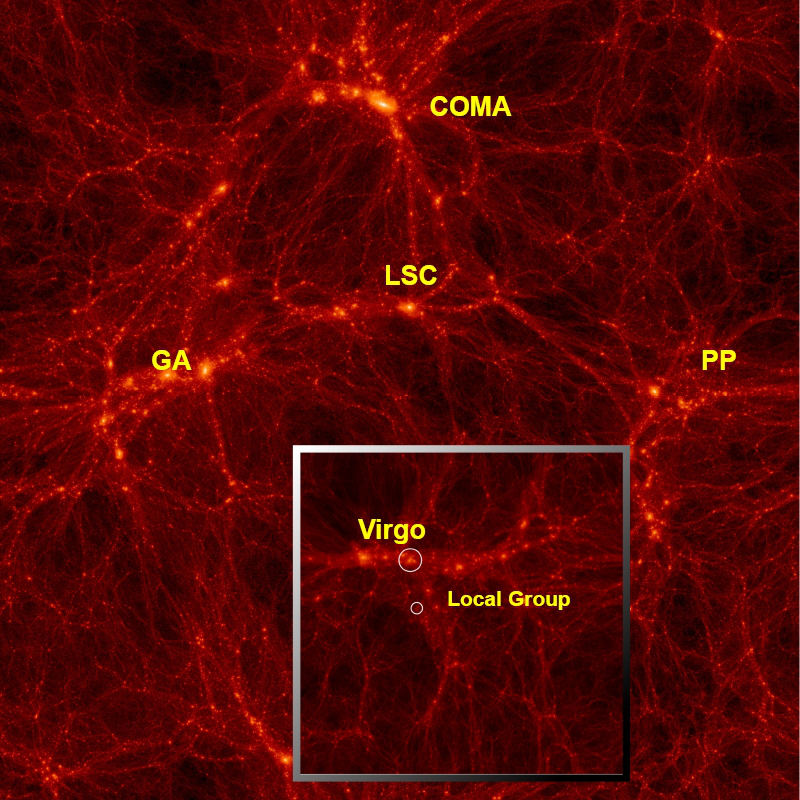
\includegraphics[width=.48\textwidth]{CLUES-DM.png}
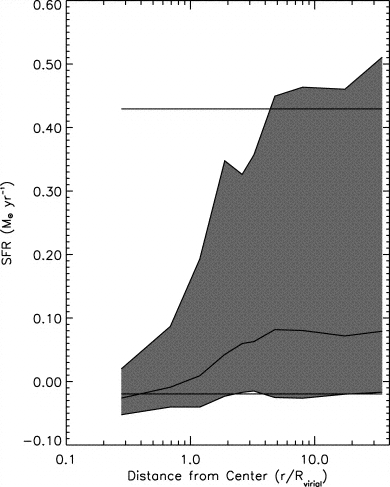
\includegraphics[width=.39\textwidth]{gomez2003-fg6a.png}
   \caption{\small  {\it (Left) } Simulation from CLUES showing
     filamentary structure surrounding clusters in the nearby
     Universe.  {\it Galaxies stream along these filamentary structures, likely sites of preprocessing.}
{\it (Right)}  Figure 6 from \citet{gomez03} showing that the upper
envelope of star formation rates begins to drop at $4R_{vir}$ from clusters.  There is a very
large scatter which complicates the interpretation of this trend.   
%Much
%of the scatter may come from the large range in local densities at a given
%projected radius due to the filamentary structure surrounding clusters.
{\it The large scatter in SFRs complicates the interpretation of this trend, and can be alleviated by studying galaxies along
filaments rather than just as a function of projected radius - this is the goal of this proposal.}}
     \label{fig1}
 \end{figure}
%In this proposal, we are focusing on where and how environment affects galaxies.  
%While interactions with the intracluster medium clearly strip gas
%from some infalling cluster galaxies \citep[e.g.][]{chung07},
%
%

{The environmental effects thus
have different signatures on the relative abundances and spatial
distribution of the warm ionized gas, neutral, and molecular gas.  By
observing both 
phases, we can distinguish among these processes.}
AGN and supernova feedback may quench star formation through
ejection or heating of the gas without impacting the distribution of
existing stars \citep[e.g.][]{springel05,
  croton06, dekel06}.  Environmentally-driven processes 
such as tidal interactions and
mergers can
affect the distribution of both gas and stars \citep{springel05,
  croton06, dekel06}, whereas pressure-driven interactions, such as
starvation \citep{Larson80} and ram-pressure stripping
\citep[e.g.][]{Gunn72}, are expected to
act primarily on the gas (see Figure \ref{decisiontree}).  
% We diagram the impact 
% For example, starvation, which results from
% a galaxy being cutoff from its supply of cold gas \citep{Larson80}, is
% expected to result in
% truncated gas disks while the spatial distribution of the
% remaining disk gas is circularly symmetric and the stellar disk is unaffected \citep[e.g.][]{kawata08}. 
% The interaction of galactic disk gas with the intracluster medium via
% ram-pressure stripping can remove the gas and produce asymmetries in
% the remaining disk gas \citep[e.g.][]{quilis00,crowl05}.  
%that disk gas is compressed in the direction of motion  and cupped in
%morphology \citep[e.g.][]{quilis00,crowl05}.  
{\bf Studying the relative distribution
and amount of gas and stars can help identify the dominant processes
that deplete gas in galaxies. }
 
\begin{figure}[h]
   \centering
 %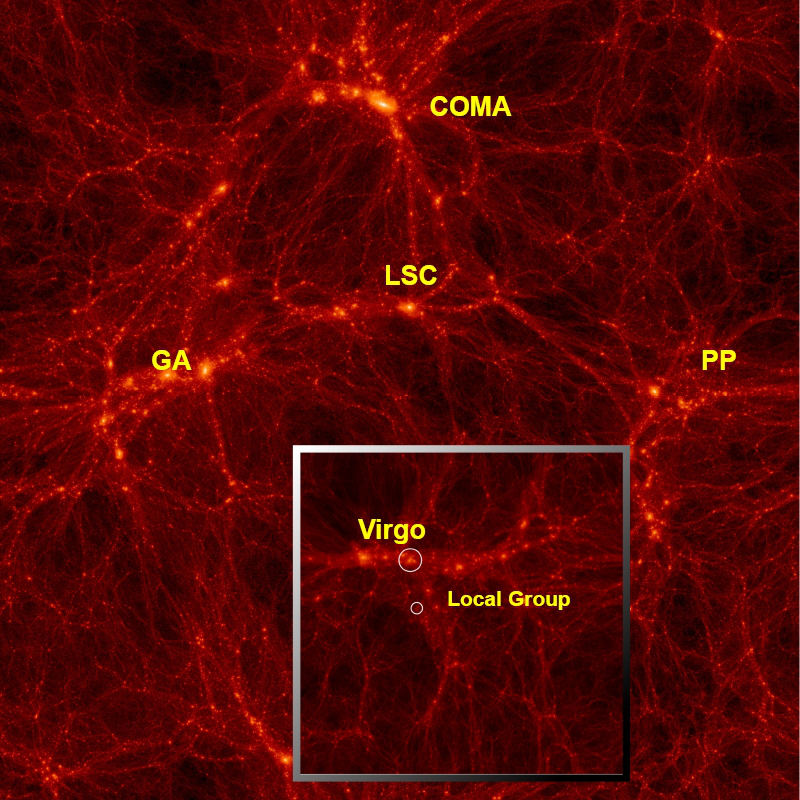
\includegraphics[width=.48\textwidth]{CLUES-DM.png}
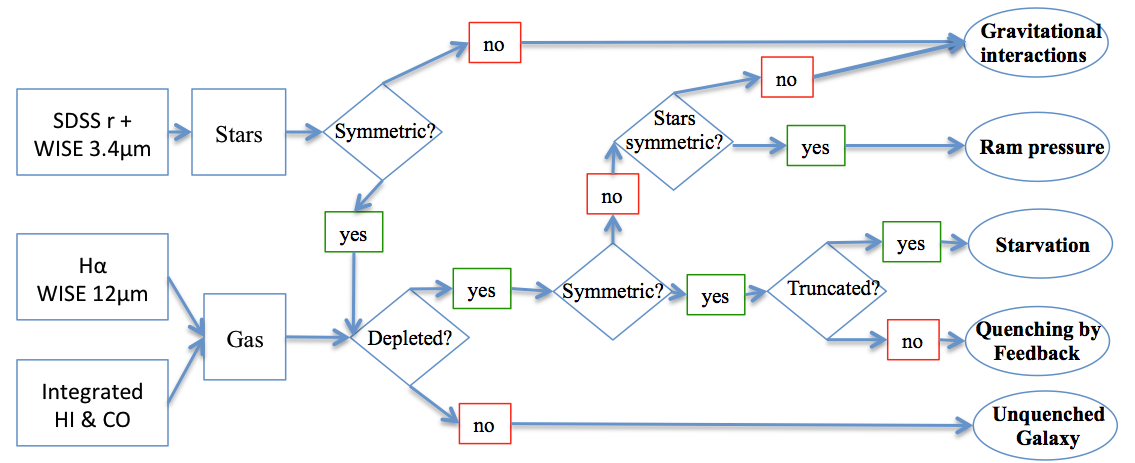
\includegraphics[width=.9\textwidth]{decision_tree.png}
   \caption{\small Our observations will test quenching prescriptions that are currently implemented in SAMs.  Current comparisons suggest that the prescriptions are incomplete (see Figure~\ref{lizhi_comparison}).  The above schematic illustrates how we can use our observational results to constrain the SAMs.  This simplified schematic does not treat the separate depletion of atomic and molecular gas and assumes that one process is dominating over the others in each galaxy.}
     \label{decisiontree}
 \end{figure}

% Large galaxy redshift surveys have revealed that galaxies are distributed in a complex network
% of matter with a large dynamic range of local density, called the
% cosmic web or filamentary structures \citep{kitaura09, darvish14}.
% These structures are seen in striking clarity in both simulations
% (left panel Fig \ref{fig1}) and around the
% Virgo cluster as shown in Figure \ref{kimfigure}.  
%Our goal is to understand how 
%galaxies are altered as they move through the cosmic web of filaments and enter the
%densest regions.  We are therefore in the midst of a
%multi-wavelength study of galaxies at a variety of positions in the
%cosmic web surrounding the Virgo cluster, one of the best studied
%regions of high density in the Universe.  

 

We have completed a survey of 200 local group and cluster galaxies, using
$Spitzer$ 24\micron \ imaging to map the spatial distribution of star
formation relative to the stellar disk (Finn et al. 2016, in prep; Local Cluster Survey - LCS).  We find that the relative
size of the star-forming disk is smaller for cluster galaxies than for
field galaxies, and the relative size of the star-forming disk
correlates with HI deficiency.  
Current semi-analytic that include starvation drastically overpredict the quenched fraction
of satellite galaxies, implying significant problems with the
implementation of environmental quenching (left panel Figure
\ref{lizhi_comparison}).  Unfortunately, the LCS data data do not probe beyond
the clusters cores, making it impossible to understand quenching in filaments.  Furthermore, due to the depth of the $Spitzer$ imaging, we are not able to probe
star formation in galaxies with $log_{10} (M_\star/M_\odot) < 9$, where the predictions of semi-analytic models diverge most
significantly from observations.


\begin{figure*}[h!]
\begin{center}
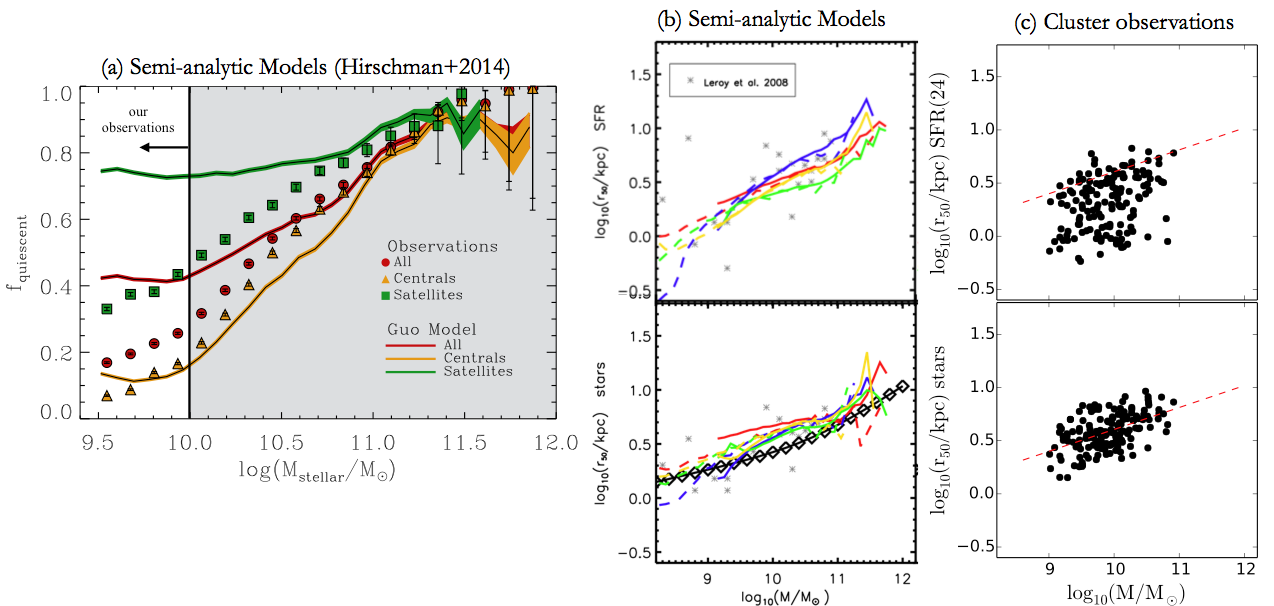
\includegraphics[width=\textwidth]{model-comparisonv2.png}
\end{center}
\vspace{-0.5cm}
\caption{\small (a) {\bf The ``satellite overquenching problem'': }  
Comparison between $z=0$ quenched fraction observations (points)
    and state-of-the-art semi-analytic model predictions (lines) from
    \citealp {guo11a} (adapted from \citealt{Hirschmann14}). This
    model, like many others \citep[e.g.][]{somerville08,kimm09},
    reproduces the quiescent fraction of central galaxies fairly well
    (yellow), but greatly overproduces the quiescent fraction of
    satellite galaxies (green).  (b)  {\bf Predicted} half-light radius
  of stars (bottom) and star formation (top) versus stellar mass for
  $z = 0 $ field galaxies (Xie et al. 2016, in prep).
  The different color lines represent different models for partitioning
  atomic and molecular hydrogen, which agree with field galaxies observations, indicated by grey points. (c) {\bf Measured} half-light radius of stars (bottom) and star
formation (top) versus stellar mass for galaxies in the {\it Local
  Cluster Sample} (Finn et al. 2016, in prep).  The
red dashed line is a linear fit to the stellar half-light radius and
is shown in the top panel for comparison.  Clearly as seen in panel a, the starvation recipes included in semi-analytic models are too efficient at quenching galaxies, but the reason is not clear.  {\it Our observations of the relative sizes of stars and gas in dense environments will provide valuable constraints for the next generation of semi-analytic models that treat environmental suppression of star formation.}}
%
%The size of the star
%forming region is smaller than predicted by semi-analytic models,
%suggesting that starvation is not sufficient to explain the observed
%size of the star-forming region in dense environments.  However, starvation greatly overproduces the fraction of quenched satellite galaxies, implying that the models are in dire need of more detailed observational constraints.}
\label{lizhi_comparison}
\end{figure*}



\vspace*{-.8cm}
\section{Our Survey of Gas in Filament Galaxies}
\vspace*{-.4cm}
This proposal builds on an existing collaboration, whose stated goal is to understand the environmental effect on gas in galaxies.  
%In this proposal we will characterize the spatial distribution of star formation in
 %low-mass filament galaxies, thus probing the mass range where quenching
 %is most effective and the environment where quenching likely first starts \citep[e.g.][]{cybulski14}. 
 Using new and archival data, we will explore the physical properties of
galaxies in the filaments around the Virgo cluster.   
While numerous studies have characterized galaxy populations within the core of Virgo, galaxies in the surrounding regions have received relatively little attention.
%
%Virgo is an ideal
%target as it is one of the best studied clusters.  However, there is
%only sparse data on galaxies in the well-defined filaments leading
%into Virgo from large radii, making our project especially timely.  
We have successfully completed the first of two awarded CO observing campaigns to directly measure the molecular gas content of galaxies within these filaments. {\it This proposal} requests funds to: \textbf{1)} obtain \ha\ observations, from which we will derive spatially resolved star formation rates of filament galaxies; \textbf{2)} produce spatially resolved dust maps with WISE 12\micron\ imaging; \textbf{3)} combine this new data set with publicly available GALEX UV fluxes,  and ALFALFA HI gas masses to characterize filament galaxies in a way that is on par with galaxies in the Virgo core. 
\begin{table}[h!]
\small
\caption{Description of Filament Galaxy Samples \label{sampletable}}
\begin{tabular}{|p{.4in}|p{.75in}|p{.3in}|p{1.6in}|p{2.6in}|}
\hline
{\bf Gas Probe} & {\bf Telescope} & {\bf$\bf  \rm N_{gal}$}& {\bf
  Mass Range} & {\bf Rationale}\\

\hline
%& & & & & \\
%\multicolumn{6}{|c|}{~} \\
%\multicolumn{6}{|c|}{\it Work Funded by This Proposal} \\
%\multicolumn{5}{|c|}{~} \\
\hline
H$\alpha$ & WIYN~0.9m, Mt Laguna & 100, 120 & $\small
8.5<\log(M_\star/M_\odot)< 10$ & mass range where environmental
effects are expected and where SAMs deviate most from observations\\
%& &120 &Rudnick & &\\
\hline
IR  & WISE & 184 & $\small 
8.5<\log(M_\star/M_\odot)< 11.5$  & all detections with $SNR(12\mu m) > 10$
 for reliable image fitting\\
\hline
%\hline
CO & IRAM & 120 & $\small 9 < \log(M_\star/M_\odot)
< 10$ & CO observations are difficult for $\log(M_\star/M_\odot)
< 9$ due to low metallicity\\
\hline
HI & Nan\c{c}ay &300&  $\small
8.5<\log(M_\star/M_\odot)< 10$ &Same as \ha \ rationale; 
75\% of sample already has HI observations from literature\\


\hline
 
\end{tabular}
\end{table}

In particular, our core comparison data set will include VLA HI gas masses (Chung et al. 2009), and Herschel and WISE infrared imaging (Davies et al. 2010) for SFRs and stellar masses.  

% \noindent \underline{The North-East Filament.} We selected the highest contrast and longest filament existing around
% Virgo. It is relatively straight over 20Mpc and extends up to 7 virial
% radii from the cluster center.  Only a small part of this filament is included in
% the Extended Virgo Cluster Catalog (EVCC), which covers 725 deg$^2$ or 60
% Mpc$^2$.  The EVCC is about 5 times larger than the surface of Virgo
% proper and extend to 3.5 virial radii, but fails to probe the extended filamentary structure around this cluster. 






% \begin{figure}[h]
% \centering
% 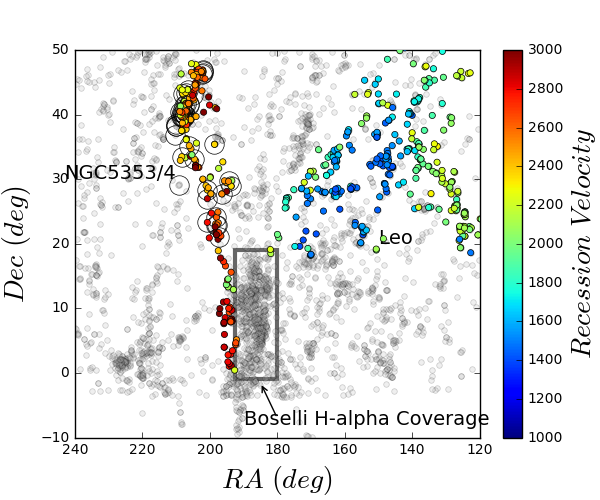
\includegraphics[width=0.6\textwidth]{filaments.png}%{Virgo_positions_NSF.png}
% \caption{%{\it (Left)} 
% Figure from \citet{kim16} showing filaments surrounding Virgo Cluster. {\it (Right)} Galaxies in the vicinity of the Virgo
% Cluster.  The main Virgo cluster is near $RA = 190$
% and $Dec = +10$. The black rectangle shows the NE filament that is the subject of this proposal.
% Galaxies in this filament have recession velocities in the range $2400 < v_r <
% 3000$~ km/s.  The gray rectangle shows the coverage of the
% Boselli large \ha \ imaging program at CFHT that will start in 2017A. It is restricted to the vicinity of the main
% cluster and will not probe galaxies along the filament where
% preprocessing is thought to happen.  The Boselli program will provide
% a useful comparison for our sample of filament galaxies.}
% \end{figure}

% \begin{figure}[h]
% %\includegraphics[width=0.48\textwidth]{Virgo_filament_Halpha_obs.eps}
% \includegraphics[width=0.6\textwidth]{Virgo_filament_CO_obs.png}
% \caption{Zoomed-in view of the filamentary structure to the NE of Virgo.
% The grey points show all galaxies in redshift range $2400 < v_r <
% 3000$~km/s.  The color points show the galaxies we are targeting
% with \ha \ emission.  These 20 galaxies will have CO observations,
% and have $S/N(22 \mu m) > 2$ and $9 < \log_{10}(M/M_\odot) < 10$;
% the points are colored according to stellar mass.
% The black squares (just slightly larger than the colored points) show the 17 HDI pointings that are required
% to image the 20 star-forming galaxies. }
% \label{fig1}
% \end{figure}



% We request time for 22 pointings in 10 groups (2 pointings for most
% groups, 
% 3 for the nearest two groups). With overhead 
% (including 5 exposures per filter to dither over MOSAIC gaps,
% pointing, and focus checks), 
% we estimate 2.5h per field = 55h for 22 fields. In addition we will
% obtain 2-3 spectrophotometric standards and 3 Landolt standard fields
% per night in each filter on photometric nights, requiring ∼0.5 hours
% per night. These observations may be carried out in astronomical twilight.
% We thus request 7 nights, assuming ∼8.5 hours of astronomical twilight per night.
% We do not require dark time for these observations, but bright
% moonlight makes it difficult to detect the outermost parts of the
% galaxies. We therefore request time at least 7 days from full moon.

 
% \ha \ falls perfectly into \ha$+4$nm.

%\vspace*{-1cm}\subsection{The Filament Galaxy Sample} 
%\vspace*{-.4cm}


\citet{tully82} first studied the large-scale structure around the Virgo
cluster and identified several concentrations of galaxies that he
termed clouds.  More recently, \citet{kim16} repeat this analysis with
a much larger spectroscopic dataset that probes to lower luminosities,
and they are able to identify multiple
filaments around Virgo (see right panel of Figure \ref{kimfigure}).
% some that lead directly into the cluster and
%others that are nearby but not falling into Virgo .
This proposal focuses on selected filaments identified by
\citet{kim16}, and we highlight these in the left panel of Figure
\ref{kimfigure}.  
The NGC5353 filament feeds the NGC5353 group and extends over 20~Mpc,
passing close to but not into the Virgo cluster \citep{kim16}.  The other filaments
that we will study feed the Virgo cluster directly.   We will therefore be able to examine galaxies feeding halos of very different masses.
%\citet{kim16} show that once
%you project galaxies into a Virgo-centric coordinate system (see right
%panel of Figure \ref{kimfigure}), galaxies
%in this region exist in three distinct filaments.  We will target all
%of these.  
We focus on
the NGC5353 and Leo filaments for two practical reasons:  (1) these filaments
extend the furthest north on the plane of the sky, and this allows
for a longer observing window from northern-hemisphere telescopes, (2)
these filaments are among the most distant in the region and
thus the galaxies have smaller apparent size, minimizing the required CO aperture corrections.

\begin{figure}[h]
\centering
%\includegraphics[width=0.6\textwidth]{Virgo_positions_boselli.png}
%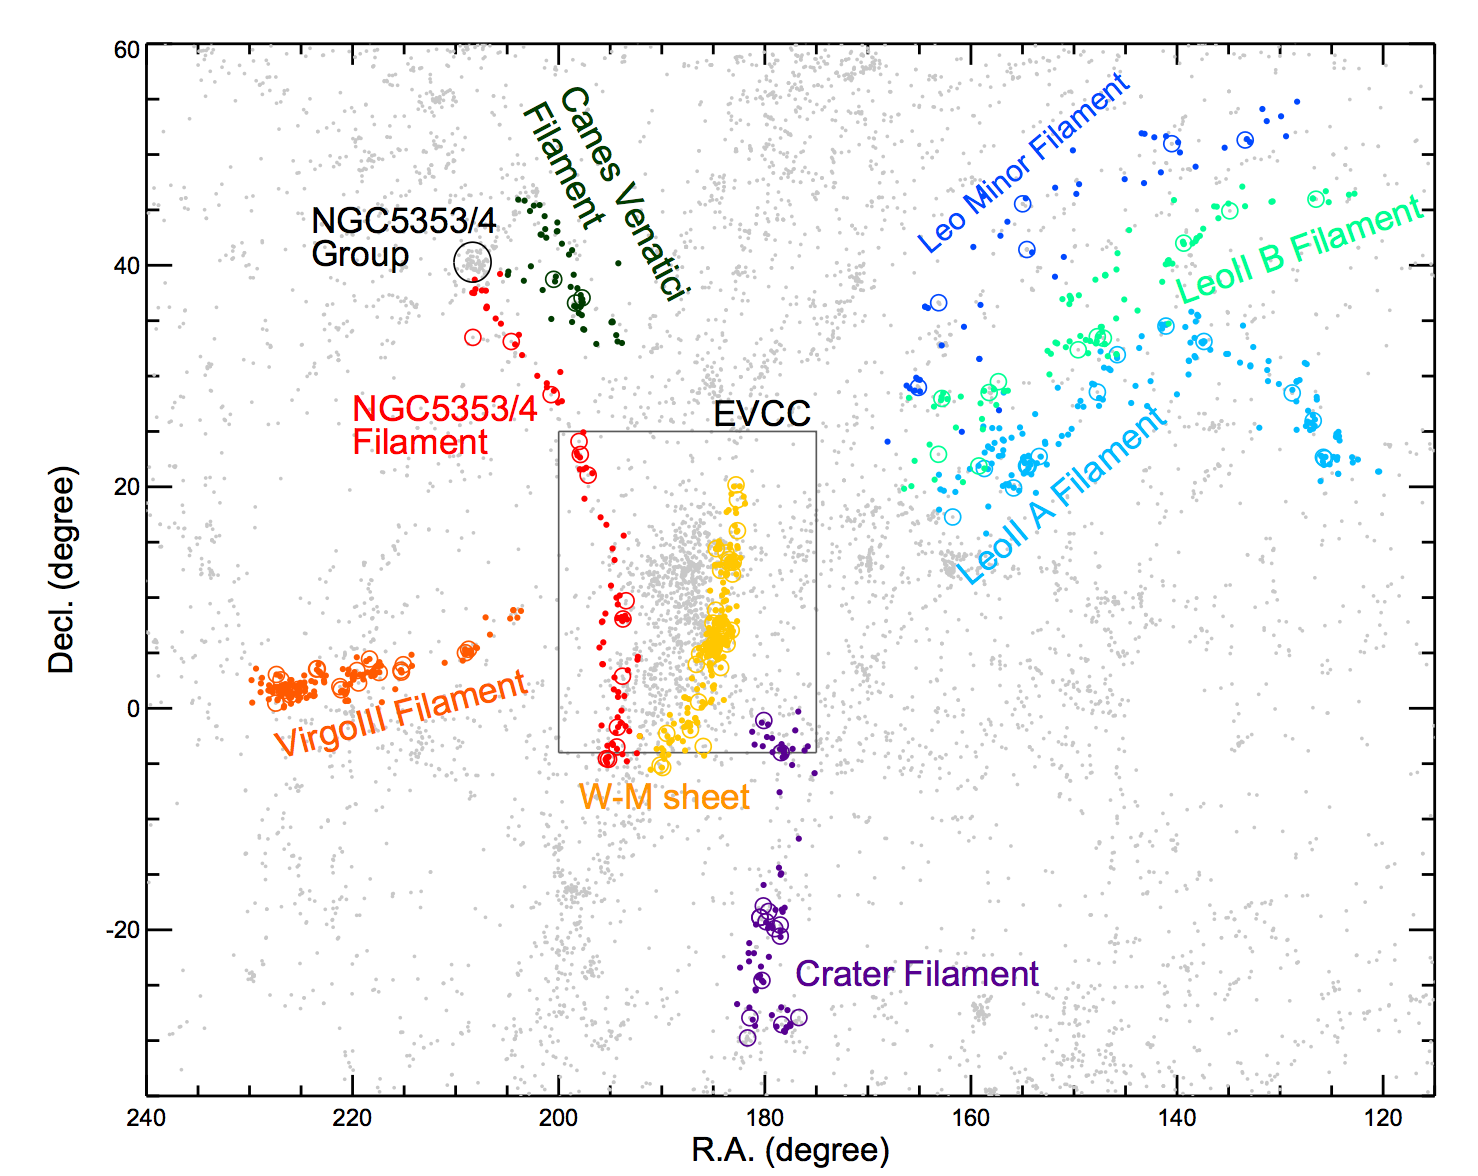
\includegraphics[width=0.48\textwidth]{KimFig1.png}
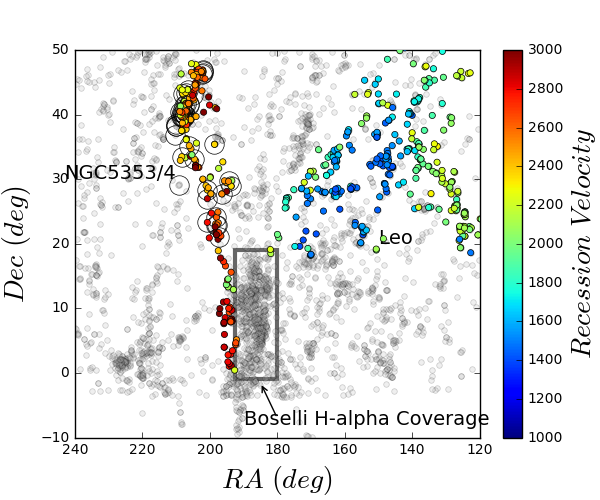
\includegraphics[width=0.5\textwidth]{filaments.png}
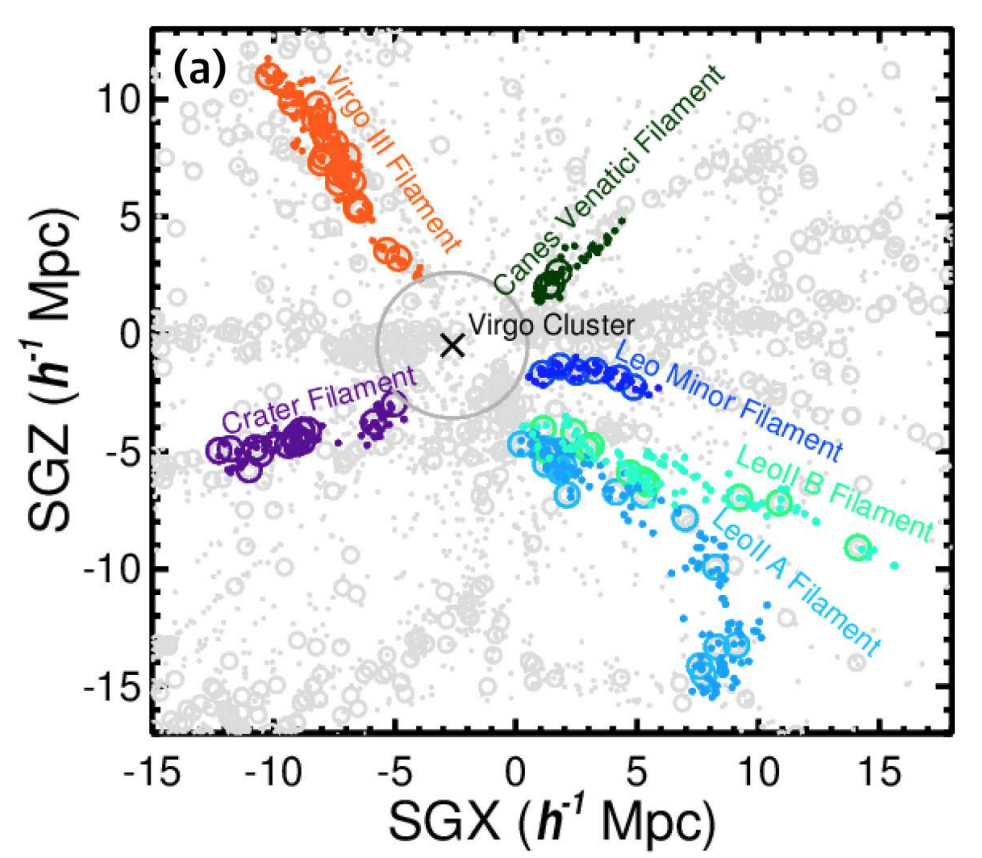
\includegraphics[width=0.46\textwidth]{KimFig2a.png}
\caption{\small {\it (Left)} Filaments as identified in Figure 1(a) of \citet{kim16} showing filaments
  surrounding Virgo Cluster as observed on the plane of the sky in RA and Dec and coded by recessional velocity.  {\it (Right)} Figure 2(a) from \citet{kim16} showing the same galaxies but projected into
Virgo-centric coordinates.  The Leo filaments can now be seen as three
distinct filaments.  The NGC5353 filament, which does not intersect
the Virgo Cluster, is not shown in the right panel.}
\label{kimfigure}
\end{figure}



The two filaments contain over 600 galaxies with a range in specific SFR and stellar mass (Figure \ref{sample}.)
 We define four subsamples of filament galaxies and describe the mass limits and rationale for
the selection of each sub-sample in Table \ref{sampletable}.
%{\bf  The acquisition, data reduction, and analysis of
%the \ha \ imaging comprise one main thrust of this proposal.
%The second main goal of this project is to map the spatial
%distribution of dust within the filament galaxies using WISE 12\micron
%\ imaging.  }


%We will complement our observations with the rich
%ensemble of data already obtained for the center of Virgo: the atomic
%gas with the VLA by Chung
%et al (2009), and also at large scale with ALFALFA \citep{giovanelli05}; the
%dust content with the Herschel Virgo Cluster Survey \citep{davies10};
%the stellar mass with WISE \citep{ferrarese12}; the recent star formation
%from UV data with GALEX \citep{boselli11}; and CFHT $H\alpha$ imaging.
%  the 120 galaxies 
%we will target with CO observations.  We have restricted the mass
%range for the CO sample to.


%We set the
%upper limit to the mass range because we expect that galaxies with
%$\log (M_\star/M_\odot) < 10$ will be most affected by the
%environment.  We will push above this mass limit as telescope time
%permits.
%The blue circles in Figure \ref{sample} show galaxies that we will
%target with \ha \ imaging.   The \ha \ subsample includes all galaxies
%with.  A total of 95 of these
%are in the NGC5353 filament and the remaining 126 are associated with
%the Leo filaments. 
%The open red circles in Figure \ref{sample} show 184 galaxies that are
%detected at 12$\mu$m by WISE with a signal-to-noise ratio above 10.
%We set this as the lower SNR limit so that we have sufficient signal for
%fitting a two-dimensional \sers \ model, and we discuss the details of
%our image fitting in Section \ref{wise}.  



\begin{figure}[h]
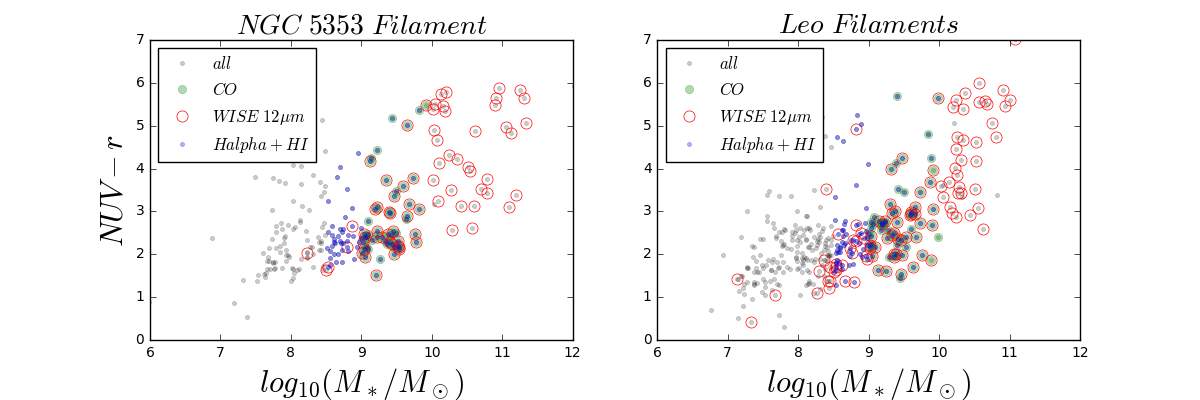
\includegraphics[width=\textwidth]{sample.png}
\vspace{-0.8cm}
\caption{\small $NUV-r$ color versus stellar mass for galaxies 
  in the ({\it left}) NGC5353 filament and the ({\it right}) Leo filaments.
Grey circles show NASA-Sloan Atlas galaxies, red circles show WISE 12\micron\ detections with $SNR > 10$,  
blue dots show galaxies that we will observe in \ha \ and HI (if
HI observations do not already exist), and green
dots show those that we will observe in CO.  The sub-samples are described in Table \ref{sampletable}.}
\label{sample}
\end{figure}


\vspace*{-1cm}\section{Proposed Work} 
\vspace*{-.2cm}
% Panchromatic galaxy surveys are required to acccurately quantify the multiple
% components of the interstellar medium (reference SINGS, THINGS, LITTLE
% THINGS), and we expect a variety of gas effects to be observable by observing a
% sample of galaxies in \ha\, HI, the mid-infrared, and CO, as described
% below.  
% Specifically, 
We will use \ha\ and WISE 12\micron\ images to measure the spatial distribution of ongoing star formation.  We will make direct measurements of the atomic and molecular gas using HI and CO data.  Finally, we will compare our observations to  theoretical models.
%We will measure the spatial distribution of
%ongoing star-formation and dust with \ha \ imaging and WISE 12\micron
%\ images, we will determine total HI and CO masses.
%Cutting off the hot gas supply or stripping the diffuse molecular gas
%is a likely precursor to the suppression of star formation as the
%galaxy will use up its cold gas on a timescale of $\sim 2.3$~Gyr
%(Bigiel et al. 2011).  Likewise, direct stripping of the cold gas will
%result in a suppression of the CO and infrared luminosity and
%truncated \ha \ emission (e.g. Koopmann et al. 2004).  
% Note that Virgo is the closest relatively massive cluster. There is no counterpart
% in which the major question of the origin of star formation quenching could be
% addressed in such exquisite details.
Below we describe our proposed work and the division of labor among the co-PIs.

% - for We take a
%similar approach, providing a complete census of warm and cold gas and
%dust.  
% We will quantify the stellar and dust components using
% SDSS imaging, optical spectroscopy, and
% far infrared (WISE) fluxes.  
% While our data is not as high resolution as the nearby data,






\vspace*{-1cm}
\subsection{Spatially Resolved Star Formation from \ha}
\vspace*{-.3cm}
%Why is \ha \ imaging important?

$H\alpha$ is the standard for measuring star-formation in local galaxies
\citep[e.g.][]{kennicutt98}, and the combination of \ha, UV, 
and mid-infrared imaging provides a powerful measure of star-formation
rates that is independent of extinction.  The
combination of star-formation rates and CO observations will allow us to calculate
gas consumption timescales and characterize multiple phases of the
galactic gas. 
Equally important, the spatial extent of \ha, when compared to the
radial distribution of the underlying stellar population and the dust (\S\ref{wise}), provides a powerful
means to identify the physical processes that affect a galaxy's gas
supply \citep[e.g.][]{hodge83, dale01, gavazzi12,boselli15}.
%and look for signatures of environmentally-driven
%depletion.
%satellite vs. central \citep[e.g.][]{omand14}.
Studies of the Virgo cluster core show evidence of cold gas stripping
\citep[e.g.][]{crowl05, chung07, corbelli12, gavazzi12, boselli15}, including truncated $H\alpha$ emission of Virgo spirals
compared with their field counterparts \citep{koopmann04}.
We will be able to determine if environmental transformation starts in
the filaments, before galaxies are accreted into the densest environments.

While extensive \ha \ imaging has been done in groups, clusters, and the field,
little has been done to map the spatial extent of \ha \ in filament
galaxies.  
The goal of our program is to obtain spatially resolved \ha \ maps for 222 star-forming galaxies in
the NGC5353 and Leo filaments. Key to testing quenching mechanisms are that we are able to measure \ha \ profiles to low surface brightness and that we can
probe galaxies at different positions along the filament out to large
distances from Virgo.
To properly probe any environmentally-driven quenching, we will detect galaxies
with star-formation rates 10 times lower than the star-forming main sequence. 
%Elbaz et al. (2011) find that a
%$\rm \log_{10}(M_\star/M_\odot) = 9$ galaxy has a SFR 
%of $\rm 0.25~ M_\odot/yr$ at $z = 0$. 
%The detection limits of our \ha \ imaging will allow us to detect galaxies with star-formation rates a
%factor of ten below the star-forming main sequence.

%\vspace{-0.3cm}
\begin{figure}[h]
\centering
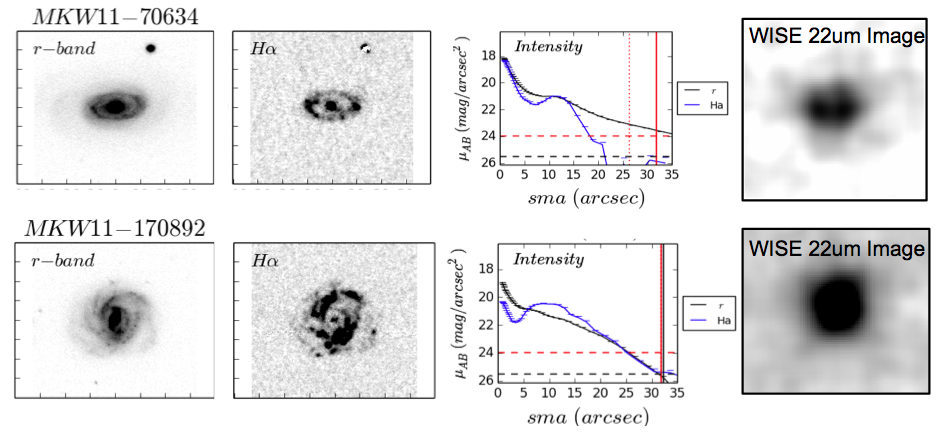
\includegraphics[width=.85\textwidth]{HalphaProfileWISE.png}
\vspace{-0.3cm}
\caption{\small
% \textit{Left:} SDSS $gri$ color composites of the 20 galaxies
%   in our $CO-H\alpha$ sample. \textit{Right:}  
To illustrate our proposed \ha \  analysis, we show
imaging taken with the KPNO 0.9-m$+$HDI of two galaxies within the
nearby group  MKW11 ($v_r = 6900$~km/s). The top row shows a
galaxy whose \ha \ is truncated
relative to the stellar disk as
probed in the $r$-band. This is clearly seen in the radial profiles (third column from left.)  The bottom row shows a galaxy with extended
\ha \ emission.  The SFR is resolved  at about 1/10 of a kpc in \ha. In
contrast, the WISE PSF at 22\micron\ is 12 arcsec, corresponding to about 1~kpc. The image thumbnails in each row are the same size, demonstrating
that the WISE data are not sufficient to measure the 
morphology of the star formation.  The WISE 22\micron\ data will be useful for a global SFR estimate when combined with GALEX UV and \ha\ imaging, and the 12\micron\ data (FWHM $=1/2$ kpc) will probe the radial profile of obscured star formation.  While the WISE photometry may
underestimate the SFR for  the lowest mass galaxies in our sample
because of their low metallicity, the combination of WISE, UV, and \ha\ imaging will allow us to understand how environment affects the distribution of star-formation.
%  As these galaxies are likely the
%most susceptible to stripping, \ha\ imaging is necessary to understand
%how environment affects their gas.
}
\label{fig3}
\end{figure}


We will complete the \ha \ observations at the WIYN~0.9 and the Phillips Claud Telescope (PCT) at the Mt. Laguna Observatory.  For the WIYN 0.9~m, we will apply for time through NOAO (already submitted a proposal for Spring 2017 semester), requesting
approximately 6 nights each spring for the three years covered by this
proposal.  Based on past \ha \ imaging experience with the WIYN 0.9~m,
we need about 2 hours per target, and so we expect to be able to
complete 4 objects per night and 24 pointings per run.  Our yield will 
be slightly higher ($\sim 30$) because we will be able to place multiple objects within
the $0.5^\circ \times 0.5^\circ$ field of view.  Thus we expect to
complete \ha \ imaging for
$\sim 100$ galaxies at the WIYN 0.9m. 

We will observe the remaining 120 galaxies in the \ha \ sample using the
PCT.  This 1.25m telescope has a 4k$\times$4k detector with a  22\arcmin$\times
22$\arcmin \ field of view.  It is in the final phase of commissioning
and should be ready for operation in Spring 2017.  The University of
Kansas is a partner on this telescope with a 15\% share of the total
time, of which co-PI Rudnick is entitled to a significant share.  This
telescope can be remotely controlled and so will allow for observing
either from KU or from Siena College; remote observing will save substantially on travel costs for such a large observing program.
% 8 hrs per night, 4 objects per night = 24 objects per run
We have included funds to purchase a narrow-band filter suitable for observing $H\alpha$  at the redshift of our filaments.  


Co-PI Finn is involved in an \ha \ imaging survey of nearby galaxy groups
as part of the Undergraduate ALFALFA Team.  She and her undergraduate
students have developed code to reduce \ha \ imaging taken with the HDI camera on
the WIYN 0.9 m telescope.  These programs will be used to reduce the
\ha \ imaging for this proposal, and we will adapt the code to
accomodate the imaging data from Mount Laguna observatory.

% Our goal is to probe galaxies with
% SFRs a factor 10 below the main sequence SFRs. 
% We convert our expected surface-brightness sensitivity to a SFR by
% first converting to a luminosity and then using the
% Kennicutt (1983) conversion:
% $\rm SFR(H\alpha)~ (M_\odot/yr)=7.9 \times 10^{-42}~L(H\alpha)~ (ergs/s)$.
% We also assume that the star formation is spread over a circular area
% of 30\arcsec \ radius (see Figure 2).  This corresponds to an integrated
% star-formation rate of $\rm SFR \approx 0.1~M_\odot/yr$.  We will
% therefore be able to detect galaxies with star-formation rates a
% factor of ten below the star-forming main sequence.
% %To select galaxies above this limit, we require a
% %WISE SNR greater than 2 at 22μm. This corresponds to a minimum SFR of
% %$\rm 0.02 M_\odot/yr$ (e.g. Chary \& Elbaz 2001).


{% \bf Fix to reflect larger sample.}
% When possible we put multiple filament targets in the same HDI
% field of view.  We are able to target the complete CO sample of 20 galaxies in 17 pointings. With overhead 
% (including 3 exposures per filter, pointing, and focus checks), 
% we estimate 2.5h per field for a total time of 42.5h. In addition we will
% obtain 2-3 spectrophotometric standards and 3 Landolt standard fields
% per night in each filter on photometric nights, requiring $\sim 0.5$ hours
% per night. These observations may be carried out in astronomical twilight.
% We thus request 6 nights, assuming $\sim 8.5$ hours of observing time per
% night.  
% We do not require dark time for these observations, but bright
% moonlight makes it difficult to detect the outermost parts of the
% galaxies. We therefore request time at least 7 days from full moon.

%\vspace*{-.4cm}\subsubsection{The Local Cluster Survey}



\vspace*{-1cm}
\subsection{Spatially-resolved Dust Emission as a Tracer of Obscured Star Formation}
\vspace*{-.3cm}
\label{wise}
WISE 12-micron images are sensitive to emission from polycyclic
aromatic hydrocarbons that are heated by young stars, and we will thus
use these images to trace the spatial extent of dust in the filament
galaxies.  
While the WISE PSF is rather large
(6.5\arcsec \ at 12\micron), it
still probes down to kiloparsec scales for galaxies in our filaments,
and is sufficient for this study (see Figure \ref{wiseCO}).   Along with SDSS fiber
spectroscopy, the WISE colors will be used to identify galaxies with an AGN.


\begin{figure}[h]
\centering
%\includegraphics[width=0.6\textwidth]{Virgo_positions_boselli.png}
%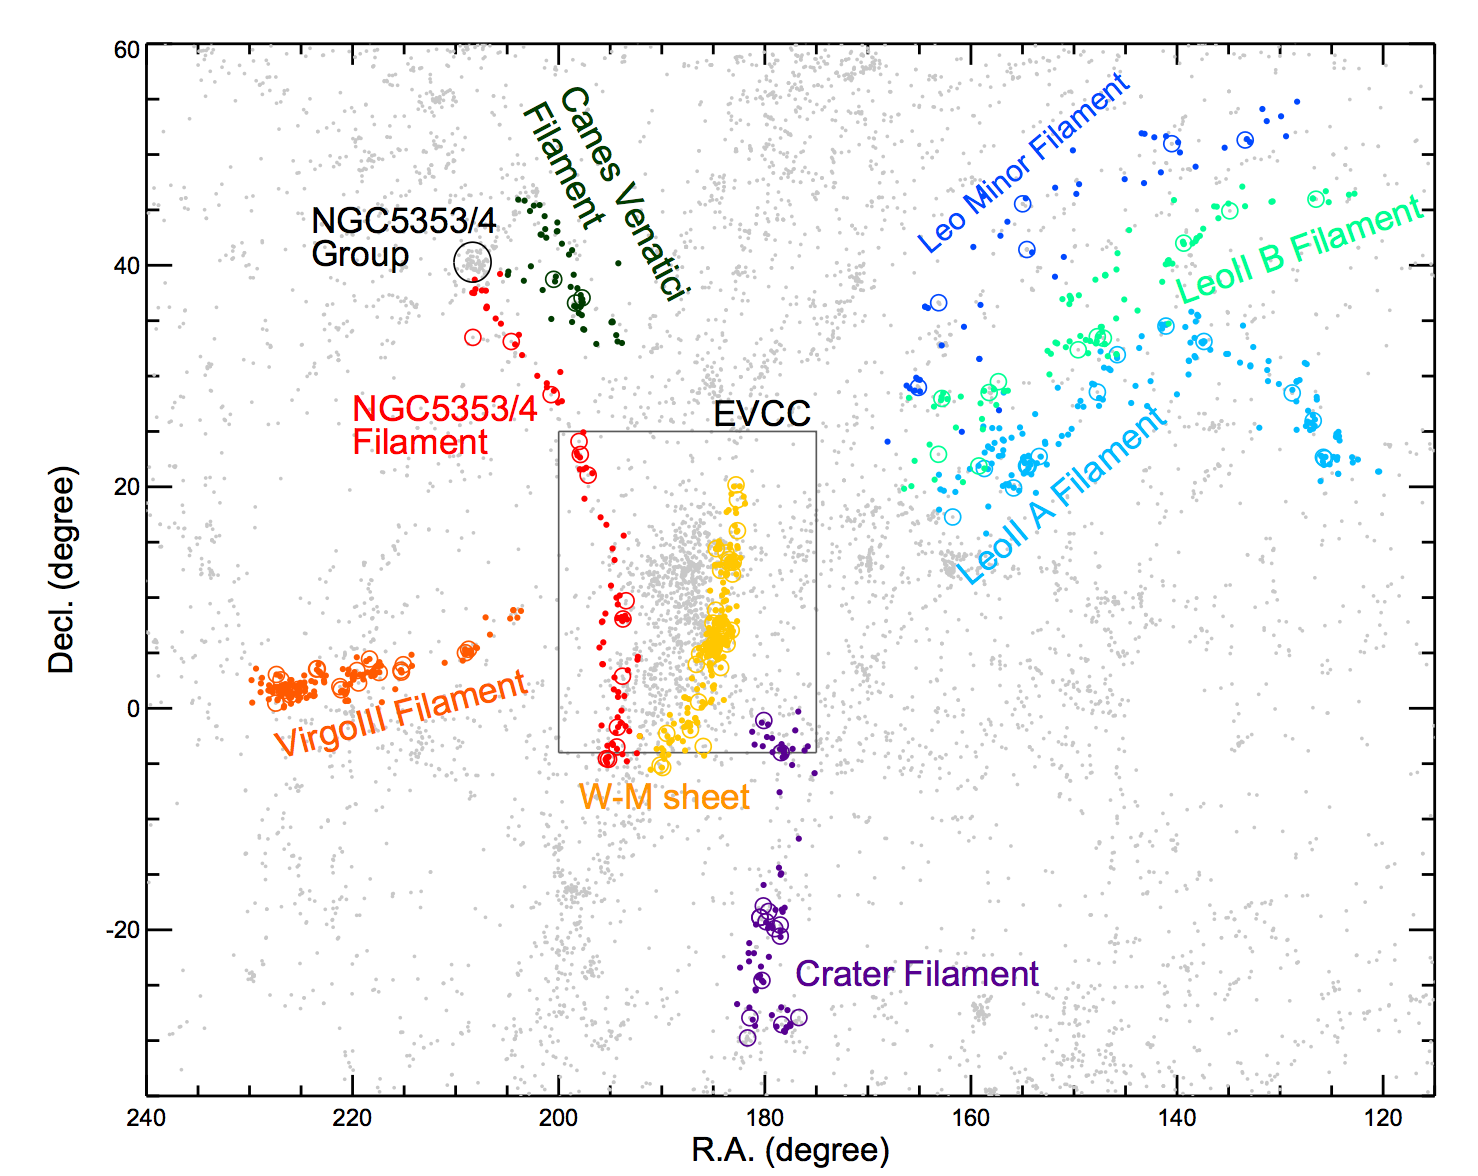
\includegraphics[width=0.48\textwidth]{KimFig1.png}
%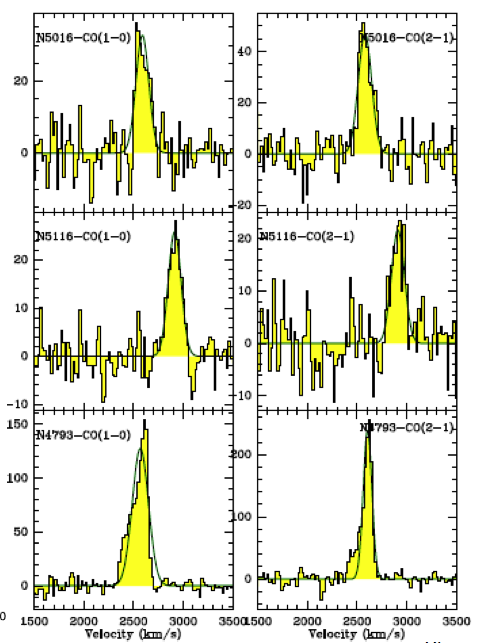
\includegraphics[width=0.4\textwidth]{CO-detection.png}
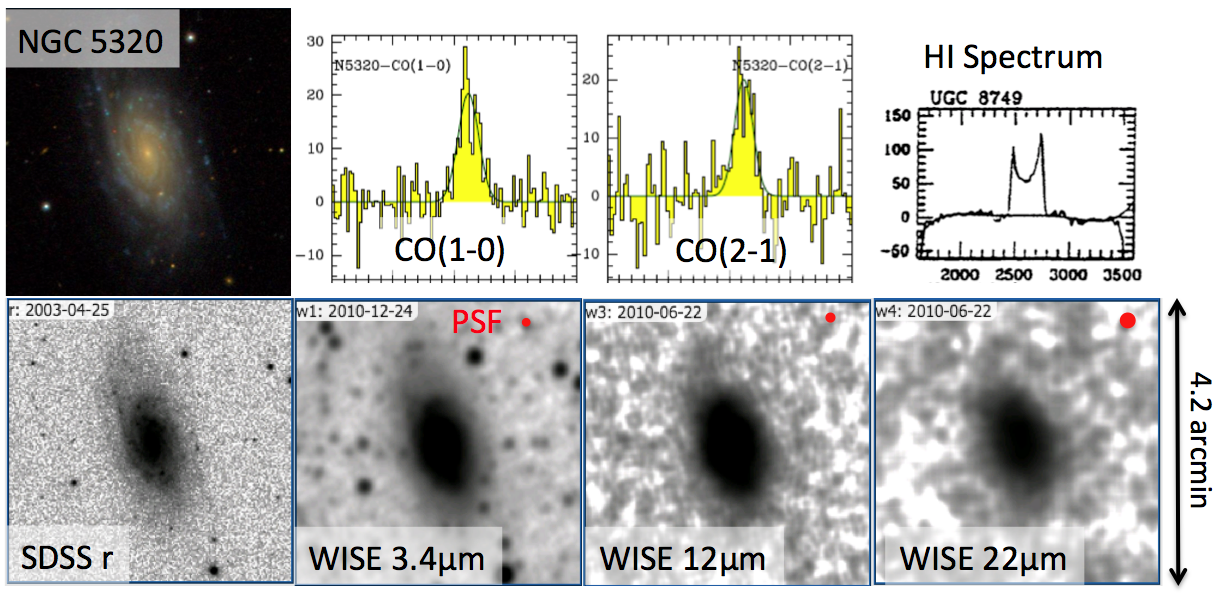
\includegraphics[width=0.8\textwidth]{NGC5320multiwaveV2.png}
%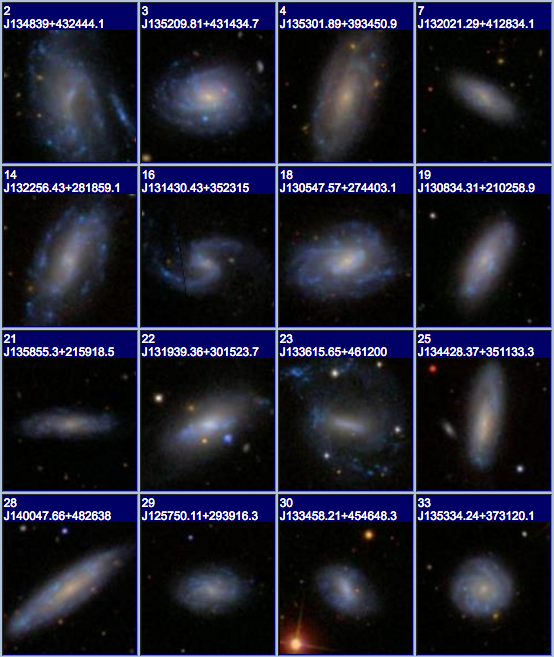
\includegraphics[width=0.48\textwidth]{sdss-montage.png}
\caption{\small 
Multi-wavelength images of spiral galaxy NGC~5320.  The top row shows
the SDSS color image, the newly acquired CO(1-0) and (2-1) spectra,
and the HI archival spectrum.  The bottom row shows the SDSS r-band
imaging and the WISE 3.4, 12 and 22\micron \ images. The resolution of WISE at 12\micron\ is
sufficient to measure the spatial extent of dust emission.  The 22\micron \ fluxes indicate the amount of
dust-obscured star formation and thus provide an important complement
to the \ha-derived star-formation rates.
% {\it (Left)} Newly acquired
%   CO (1-0) and (2-1) spectra
%   from IRAM 30-m telescope for galaxies in the NGC5353 filament taken
%   during October 2016.  Of the 40 galaxies that were observed, 38 were
% detected in CO.  Collaborator Jablonka will observe an additional 40
% galaxies in December 2016, and she will continue observations until
% the CO sample is complete.
% {\it (Right)} SDSS color images showing 16 randomly
%   selected galaxies in NGC5353 filament.  
}
\label{wiseCO}
\hrule
\vspace{-0.5cm}
\end{figure}

% This proposal rests on the assumption that 12\micron \ emission, in
% the absence of an active galactic nucleus, traces the star-forming and
% thus gas-rich regions of a galaxy.  This is clearly the case for
% 24\micron \ emission \citep[e.g.][]{calzetti07}, and so here we show
% evidence that the 12\micron \ emission (1) is comparable in extent to the
% 24\micron \ emission, and (2) can differ significantly from the stellar
% disk in terms of extent and morphology. 

% we provide a qualitative example.  In Figure
% \ref{nsa88353}, we show a spiral galaxy with 12\micron \
% emission that is comparable in extent to the stellar disk.  Again,
% comparing the $r$ and 24\micron \ images shows a more extended
% star-forming disk, and the best-fit \sers \ models indicate that the
% 24\micron \ emission has an effective radius that is 90\% of the
% stellar radius.  Importantly, the 12\micron \ emission is again
% comparable in extent to the 24\micron \ emission.


% \begin{figure*}[h]
% \begin{center}
% 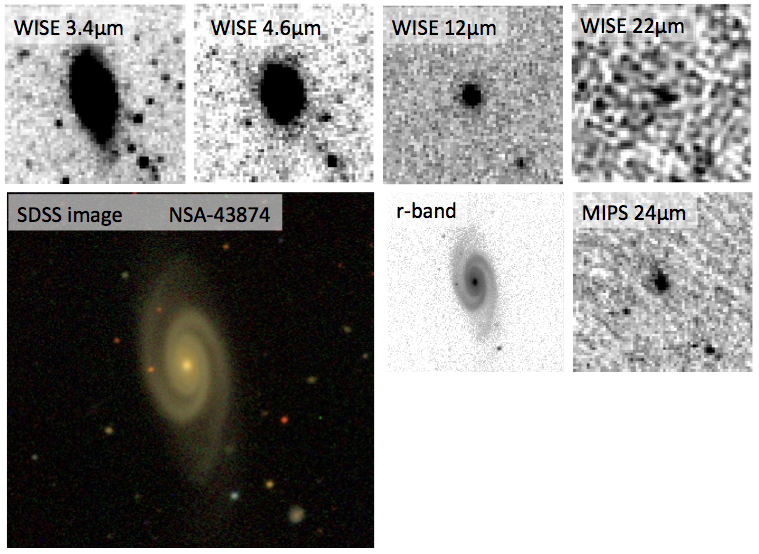
\includegraphics[width=.85\textwidth]{NSA-43874.png}
% \end{center}
% \caption{ Multi-wavelength images of spiral galaxy NSA-43874.  The top
%   4 panels are the WISE images.  The second row shows, from left to
%   right, the SDSS color, SDSS $r$, and MIPS 24\micron \ cutouts.  This
% galaxy has 24\micron \ emission that is truncated relative to the
% stellar disk ($r$-band).  The 12\micron \ emission is comparable in
% extent to the 24\micron \ emission and thus makes a suitable probe of
% the star-forming disk.}
% \label{nsa43874}
% \end{figure*}

% \begin{figure*}[h]
% \begin{center}
% 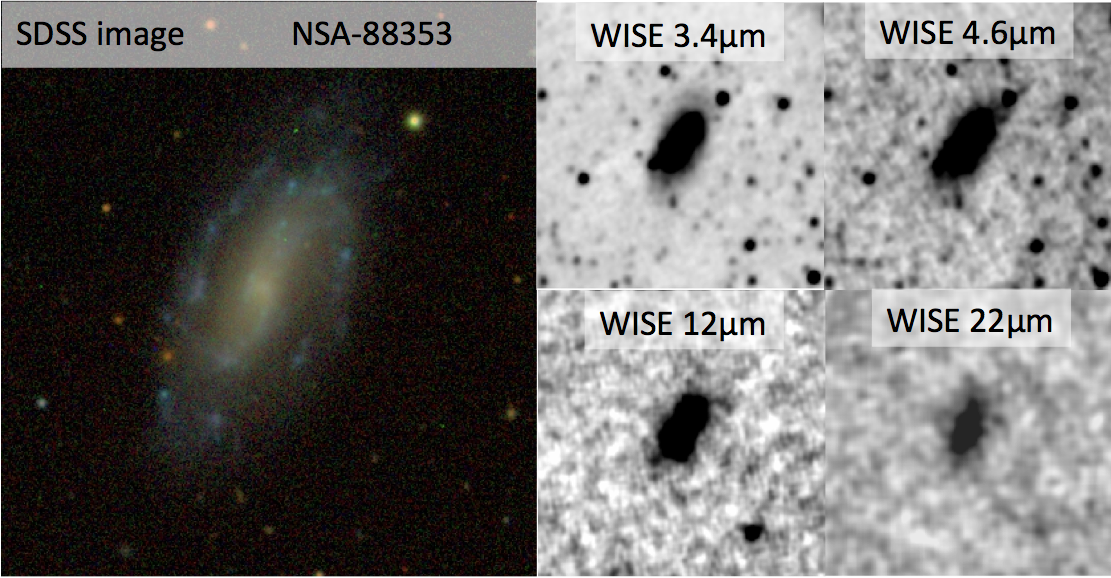
\includegraphics[width=.85\textwidth]{NSA-88353.png}
% \end{center}
% \caption{ Multi-wavelength images of spiral galaxy NSA-88353.  The 
%   4 panels on the right are the WISE images. The resolution of WISE is
% sufficient to measure the spatial extent of dust emission using the
% 12\micron \ images.  The 22\micron \ fluxes indicate the amount of
% dust-obscured star formation and thus provide an important complement
% to the \ha-derived star-formation rates.}
% \label{figwise}
% \end{figure*}

% The above examples show qualitatively that the 12 and 24\micron \ emission
% have a similar spatial extent.  To provide a quantitative example, 
% we show a preliminary GALFIT analysis for the 12\micron \ image of one spiral
% galaxy in Figure \ref{nsa113482}.  The top panel shows the results for
% the 12\micron \ image, and the bottom set of images shows the best-fit
% for the 24\micron \ image.  The best-fit models, shown in the center
% panels, have effective radii that agree within the errors.  Thus, we
% conclude that the
% 12\micron \ images provide a suitable means of tracing the extent of
% the star-forming disk.   

% \begin{figure*}[h]
% \begin{center}
% 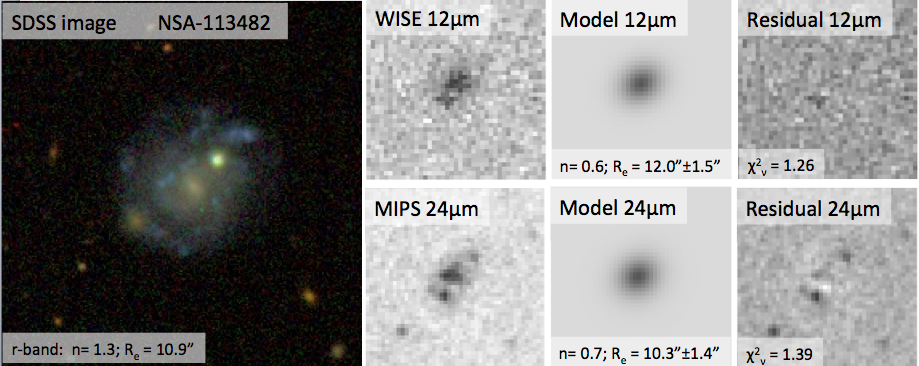
\includegraphics[width=.85\textwidth]{NSA-113482.png}
% \end{center}
% \caption{ Color SDSS image of spiral galaxy NSA-113482 (left).  The top
%   row of three images shows the preliminary GALFIT
%   analysis for the 12\micron \ image (top row).  The three images show
% the 12\micron \ image (left), the GALFIT model (center), and the
% residual after the model is subtracted from the image.  The bottom
% panels show the same for the MIPS 24\micron \ image.  The model panels
% list the \sers \ profile and effective radius of the best-fit model,
% and the effective radii from the 12 and 24\micron \ fits agree within
% errors.  This shows that 12\micron \ is a suitable means of tracing
% the extent of the star-forming disk.}
% \label{nsa113482}
% \end{figure*}


To quantify the extent of the WISE 12\micron \ images, 
we will use  {\it GALFIT} software \citep{peng02}
to fit two-dimensional \sers \ models to the galaxy images.  We will use {\it unWISE} image products and PSFs \citep{lang14}
because they are optimized for extended sources whereas the WISE
image products have been optimized for point sources.
Co-PI Finn has completed a similar analysis using GALFIT to analyze MIPS
24\micron \ images for galaxies in 9 nearby galaxy clusters (Finn et
al. 2016, in prep).  The
spatial resolution of the MIPS 24\micron \ images is comparable to the
resolution of WISE at 12\micron, yet the filament galaxies are
significantly closer than the galaxies that we analyzed with MIPS.  We have also performed extensive simulations to show that we can recover sizes for galaxies with WISE 12\micron\ SNR$>10$.  
We are thus confident in our ability to measure robust sizes at 12\micron.  


% GALFIT requires a PSF image to properly model galaxies, and this is
% particularly important when modeling low-resolution data such as the
% 12\micron \ images.  We will use a nearby point source for each
% galaxy, choosing a bright, isolated source that shows a
% clear diffraction pattern.



%We will use {\it unWISE} image products and PSFs \citep{lang14}
%because they are optimized for extended sources whereas the WISE
%image image products have been optimized for point sources..
%We will use the best-fit parameters from the $r$-band as the initial
%guess for the 12\micron \ fits. To test the sensitivity of our results to these
%initial conditions, we will stochastically vary the intial
%conditions to provide more robust estimates of range of acceptable
%fit parameters.  This process is described in more detail below.
%The WISE  data have lower resolution and
%lower signal-to-noise ratios than the optical imaging that
%GALFIT is typically used with. 
%We will use simulated galaxies to test the reliability of our GALFIT
%model parameters.
% and determine the
%surface brightness limit of our survey.

%Siena College has recently acquired a High Performance  Computer
%Cluster  (described in Facilities). 
%he cluster %, which is geared primarily towards research
%activities, represents a joint venture by Chemistry, % (Prof. G. Barnes),
%Physics, % (Prof. G. Vernizzi, Prof J. Moustakas) 
%and Computer Science.  %(Prof. Small Research Groups).  
%It 
%consists of 16 nodes each with two
%Intel Xeon E5-2630 6-core processors and 32 GB of RAM.  The cluster
%has a total global storage capacity of 20.5 TB and 208 cores each
%running at 2.3 GHz.  
%Several scientific computing software packages
%are installed on the cluster, such as Gamess, NWChem, Gromacs, LAMMPS,
%Octave, Scilab, FFTW, and MySQL Cluster.  In addition T
%The Intel
%compiler suite is available to create efficient custom programs.


The analysis of the WISE imaging will be the most computationally
intensive part of the proposed work because we plan to run multiple
models for each galaxy to assess the impact of our initial conditions
on the resulting size measurements.  For each galaxy, we will
stochastically sample across the parameter space of initial
conditions, and each model has five free parameters.  Nonetheless,
using extensive testing, we estimate that it would take less than 2
days of computational time on the Siena College High Performance
Computer Cluster (HPCC, see Facilities section of this proposal).  Co-I Vernizzi will be responsible for this piece of the project. We will compare the GALFIT results to those
generated by other independent fitting programs such as  GALPHAT \citep{yoon11} and The Tractor \citep{lang16}.

%We estimate the computational
%complexity for analyzing the WISE images for $\sim 200$ galaxies with
%GALFIT in a systematic fashion.  We would scan over the
%five-dimensional parameter space p$=$(x, y, radius, concentration,
%brightness), by discretizing each dimension between a minimum and a
%maximum value. Assuming an average of 10 points per search direction,
%the discrete lattices has $10^5$ points. Preliminary analyses show
%that the average time GALFIT takes to fit each WISE image is about 20
%seconds. That corresponds to a total estimated computational time of
%the order $4 \times 10^{8}$ seconds to scan the entire parameter
%space, which can be managed by the High Performance  Computer Cluster
%(HPCC, see Facilities section of this proposal) available at Siena
%College (in about a couple of weeks of computational time). However,
%additional fine tuning of the parameters (e.g. by
%doubling the number of lattice points per parameter dimension) can
%quickly lead to a system that is beyond to Siena College’s current
%computational capabilities.  For that reason we plan to perform a
%stochastic sampling of the parameter space, with GALFIT.  In fact,
%since GALFIT’s minimization algorithm is based on a quadratic function
%(by means of the Levenberg-Marquardt algorithm), we can estimate the
%Hessian numerically around randomly chosen starting points $\{p\}$
%from which we can extrapolate the size of the basin of attraction (the
%\sers \ model requires an initial guess for the center (x,y),
%effective radius, \sers \ index, and magnitude) . A similar strategy
%has been successfully adopted in \citep{pardo11} where Monte Carlo
%sampling alternates with gradient minimization algorithm.  By running
%it on Siena College’s HPCC, we estimate it would take less than 2 days
%of computational time. The test and exploratory runs are anticipated
%to take an additional 50 CPU hours \citep[for a recent application of
%this method see,]{sala12}. The two computational techniques described
%above are sufficient to create a map of the full phase diagram
%accurately.  In addition, we will compare the GALFIT results to those
%generated by other independent fitting programs such as  GALPHAT
%\citep{yoon11} and The Tractor \citep{lang16}.


%Use our CO observations and those from the literature to calibrate the
%use of WISE profiles as the tracer of the dense gas.  


\vspace*{-1cm}
\subsection{Molecular and Atomic Gas}
\vspace*{-.3cm}



% HI observations are already available in the literature for 75\% of
% these galaxies and we are proposing to get the remainder using the
% Nan\c{c}ay telescope, which has a low oversubscription.

The CO luminosity can be used to estimate the molecular Hydrogen mass
that is the direct fuel for star formation.  The conversion from CO
luminosity to to H$_2$ mass depends on metallicity, which in turn
depends on stellar mass, as well as on parameters such as cloud size,
which scale with the SFR density.  This conversion has been calibrated
both observationally and theoretically (see \citet{Bolatto13} and
references therein), and we will use it to estimate the molecular gas
mass of our galaxies.  This is crucial to understand how the moderately dense gas is affected by environmental gas processes.

Team members Jablonka and Combes are leading the observing campaign to
measure CO(2-1) and (1-0)  for all filament galaxies with $9 <
\log_{10}(M_\star/M_\odot) < 10$ using the IRAM 30-m telescope.
Galaxies below this mass limit are difficult to detect in CO due
to lower metallicity and photodissociation of CO
\citep[e.g.][]{cormier14}.   During October 2016, they succesfully observed 40 galaxies in the
NGC5353 filament, and 38 of these were detected.  We show the CO
spectra for one of these detections in Figure
\ref{wiseCO}.  The team has an additional block of time in December
2016, and we expect to double the number of CO detections.  Jablonka
and Combes will continue to apply for IRAM time to complete the CO observations.

We will use HI to trace the more diffuse gas.  As it is optically
thin, it is also trivial to convert an HI luminosity to a neutral
Hydrogen mass.  Finally, HI typically has a much larger radial extent
than CO and as a result is more sensitive to environmental effects.  
% and my provide
%evidence of the external gas supply being cut of (starvation).   
75\% of our target galaxies already have HI observations, and collaborators
Jablonka and Combes are leading the effort to observe the remaining galaxies.
We have submitted a proposal to use the Nan\c{c}ay $\rm 200 \times 35~m^2$
telescope, which has a low oversubscription rate and to which Combes
and Jablonka have
preferred access.  We will continue to request time on this telescope
until the HI observations are complete (see letter of collaboration).

With the HI and CO observations of our targets we will accomplish the following immediate goals: 
(1) We will measure their total molecular and neutral gas content; (2)
we will compare the atomic and molecular content as different gas
depletion mechanisms affect the diffuse and dense gas differently; (3)
we will compare this to the galaxy sizes, SFRs, and stellar masses to
determine the gas deficiency of filament galaxies (if any) compared to
galaxies in the field, group, and clusters with similar data as
obtained from the literature 
\citep[e.g.][]{Ciesla12, davies10}.


%{\it can we use this anywhere?} 

\vspace*{-1cm}
%\subsubsection
\subsection{Comparison with Theory}
\vspace*{-.4cm}

An important aspect of our work is using theoretical models to understand what processes are affecting the gas distribution in our galaxies.  Our collaborator De Lucia is an expert in semi-analytic models of galaxy formation and, in addition to her existing models \citep{Zoldan16} will produce models directly suited for comparison with our observations.  The first scenario we must consider is whether our results are
consistent with predictions of gas depletion through starvation and
the consumption of the remaining gas
rather than more extreme environmental processes such as ram-pressure stripping.
In the middle panels of Figure \ref{lizhi_comparison}, we show the predicted size of the
stellar and star-forming components of $z = 0$ galaxies based on the
semi-analytic models of Xie et al. (2016, in prep).  These models
include starvation but do not explicitly include environmental
processes such as ram-pressure stripping.  However, these models are largely untested in dense environments.  In the right panel of
Figure \ref{lizhi_comparison}, we show the {\it measured} size of the
star-forming and stellar disks versus stellar mass for the {\it Local
  Cluster Survey} galaxies (Finn et al. 2016, in prep).  We will use the measured size of star formation in filament, group, and cluster galaxies to constrain the environmental gas processes included in the models.    
%  While the size of the stellar disks are
%consistent with the model predictions, the size of the star-forming
%regions fall systematically below the model predictions.  This
%indicates that additional environmental processes must be included to
%explain the small observed size of the star-forming region in these
%galaxies.  
While providing useful data for this exercise on the cores of clusters, the {\it Local Cluster Survey} sample is small and does not probe filamentary structures surrounding the clusters.


%However, the {\it Local Cluster Survey} sample is small and
%contains very few isolated/field galaxies.
%We need (1) a larger sample of cluster galaxies to confirm the inconsistency between model
%and obervations, (2) a larger field sample to serve as a controlled
%comparison with the models, and (3) a more robust determination of
%the size of the star-forming region that includes a formal analysis of
%uncertainty.



Theoretical models of ram-pressure stripping provide predictions that
we can compare directly to our measurements.
For example, numerical simulations of starvation and ram-pressure stripping of cold gas 
generically predict that star formation in the edges
of galaxies will be affected more strongly than star formation near the
centers of galaxies; the spatial extent of the star-forming disk
should be smaller for galaxies that are undergoing stripping \citep[e.g.][]{kawata08, bekki14}.
We find evidence of this in the {\it Local Cluster Survey}, but we
also find a stronger correlation with bulge-to-total ratio.  A large sample that extends beyond the virial radius of clusters is needed to disentangle these effects and this sample has to have low stellar mass, as those galaxies should be more
vulnerable to having their gas removed 
because their gas is not as tightly
bound \citep[e.g.][]{kawata08, mccarthy07, bekki14}.

%A larger
%sample is needed to disentangle these effects.
%In addition, low mass galaxies should be more
%vulnerable to having their gas removed 
%because the gas in lower mass galaxies is not as tightly
%bound \citep[e.g.][]{kawata08, mccarthy07, bekki14}.  We find
%some evidence of this in the {\it Local Cluster Survey}, but a larger
%sample is needed to strengthen the statistical significance. 

The SAMS implemented for many clusters in the Millennium simulation
and in cluster zoom simulations will give us a statistical view of how
galaxies are affected in filaments around clusters and groups of
similar mass to Virgo and NGC 5353.  However, none of these clusters
actually looks like the surroundings of Virgo, which introduces a
systematic error in the comparison.  We will therefore implement our
SAMS in the Constrained Local UniversE Simulations (CLUES) of the
local volume \citep{Carlesi16}.  Specifically, Co-I De~Lucia will work to integrate her SAMS with the
CLUES  dark matter merger trees so that she can predict the spatial
distribution of star and star formation for galaxies in a simulation designed to look like the local volume.

\vspace*{-.9cm}\subsection{Workplan \& Personnel}
\vspace*{-.3cm}

% Justify collaboration - greg brings telescope access and resources,
% environment studies.  Finn brings expertise of IR imaging fitting, spatially resolved SF
% and \ha \ imaging observations and reduction.

The division of observing and analysis responsibilities among the team
members is outlined in Fig.~\ref{fig:workplan}.   The expertise and
roles of individual team members is described below.

Rose Finn, Ph.D., (co-PI) is a professor in the Department of Physics
and Astronomy at Siena College (Loudonville, NY).  She is the PI of
the \lcs \ and has extensive experience with running GALFIT on MIPS
24\micron \ imaging.  She will lead the \ha \ imaging survey at KPNO
and the analysis of the WISE 12\micron
\ imaging, supervise the undergraduate students.  %, and draft the paper.

Gregory Rudnick, Ph.D.,  (co-PI) is an associate professor at the University of
Kansas.  He has expertise in galaxy evolution and the effects of environment on galaxy evolution, and he is leading an
$HST$ study to measure the spatial extent of star-formation in
intermediate-redshift galaxies.  He will lead the \ha \ imaging survey
at the PCT and will supervise the graduate student whose Ph.D. dissertation will be on this project.

% Vandana Desai, Ph.D., is an astronomer at the NASA/IPAC Infrared
%   Science Archive (IRSA).   Vandana has extensive experience
% in all aspects of infrared astronomy and will lead technical aspects
% associated with the WISE data.  
% She also is well-versed in best-practices of data sharing and will
% lead our efforts to disseminate data products over the web.

Graziano Vernizzi, Ph.D., is an associate professor at the Department of
Physics and Astronomy of Siena College (Loudonville, NY).
%He has held research positions at the Department of Materials Science
%and Engineering of Northwestern
%University (Evanston, IL), at the Institute of Theoretical Physics
%IPhT) of CEA/Saclay (France), and at the Physics Department of
%University of Oxford (Oxford,UK). In 2007, he received the Cozzarelli
%Prize from the editors of the Proceedings of the National Academy of
%Sciences (PNAS) for the best article in Engineering and Applied
%Sciences. 
His research interests lie in computational and theoretical
physics, biophysics, nanoscale science, soft condensed matter, and
random matrix theory. 
%Recently, he published a chapter in the The
%Oxford Handbook of Random Matrix Theory (Oxford University Press,
%2011) on the application of random matrix theory to the study of
%ribonucleic acid folding.  
Graziano will the lead the computational
aspects of this project.



% Gabriella De Lucia, Ph.D, is a permanent research scientist at INAF -
% Astronomical Observatory of Trieste.  Grabriella provides expertise in
% semi-analytic modeling of galaxy evolution. She is working on models
% that predict the spatial extent of the stellar and star-forming disks,
% and her work is thus extremely pertinent to this proposal.  She will lead
% the theoretical interpretation of our results and the comparison
% with semi-analytic models of gas consumption.

% Pascale Jablonka is senior researcher at the Laboratory of
% Astrophysics of EPFL (Switzerland). She conducts both observations and
% numerical simulations to gain insights into the formation and
% evolution of galaxies. Her research focuses on two mains
% topics related to the present proposal: i) Infering the driving
% parameters of the galaxy star formation histories. ii) Deciphering the
% impact of the environment on galaxy evolution. She is leading a CO
% survey of cluster galaxies at intermediate redshift. She will observe
% the cold gas content of galaxies in the filamentary structures feeding
% the Virgo cluster, in atomic (HI) and molecular (CO) forms.


% Francoise Combes, PhD, is a Professor at College de France, and astrophysicist at Paris Observatory. She is an expert in the dynamics of galaxies, their star formation (SF) efficiency and feedback processes, including the action of a super-massive black hole. She has made numerical simulations to test the processes of SF quenching, ram pressure stripping, tidal interaction, or strangulation. She will observe the cold gas content of galaxies in the Virgo filaments, the atomic (HI) or molecular (CO) reservoirs.



% A total of 12 Siena College undergraduates students will be involved
% in this project over the course of three summers.  During the first
% summer, the students will work on cross-matching our galaxy sample
% with ALFALFA, GIM2D structural fits, and the unWISE photometric catalogs.  During the second summer, the
% students will analyze the star-forming main sequence using the
% WISE-derived star-formation rates.

%\begin{table}[h!]
\small
\caption{Major Milestones and Schedule \label{schedule}}
\begin{tabular}{|p{.5in}|p{.5in}|p{1.4in}|p{1.in}|p{1.in}|p{1.2in}|}
\hline
\multicolumn{2}{|c|}{\bf Timeline} & \multicolumn{3}{|c|}{\bf Responsibilities} & {\bf Dissemination} \\
\hline
 \multicolumn{2}{|c|}{~~} & Finn & Desai & Vernizzi & \\
\hline
%& & & & & \\
{\bf Year 1 (2017)}& Spring & Finalize sample selection; identify and remove AGN; write code to retrieve cutouts from {\it unWISE}; calculate stellar masses & 
Identify best techniques for modeling WISE PSF & 
Adapt GALFIT code to run on Siena computer cluster; develop code to run image analysis on parallel computing system & \\
\hline
 & Summer & Supervise summer students - cross match sample with other surveys (ALFALFA, GIM2D, unWISE photometry); identify groups and clusters within survey region; calculate environment parameters such as local density & 
Fit IR templates to estimate IR luminosity and SFRs for galaxies & 
Run code on computer cluster for a subset of the sample; adjust code and methodology as needed & \\
\hline
& Fall & Cross-check results with size measurements from MIPS data; run simulations to understand reliability limits &
Interface with NED to plan for web release & 
Run code on complete sample & \\
\hline
{\bf Year 2 (2018)} & Spring & \multicolumn{3}{|c|}{Continue with analysis of full sample.} & 
Poster at Jan 2018 AAS on preliminary results \\
\hline
& Summer & Finalize analysis; supervise summer students (star-forming main sequence as a function of environment);
draft paper &
Help draft paper; supervise web dissemination & 
Help supervise summer students; help draft paper & 
Make data products publically available through NED \\
\hline
& Fall &  \multicolumn{3}{|c|}{Continue with analysis of full sample.} & 
present results at topical meeting;
publish paper; release data to web \\
\hline
\end{tabular}
\end{table}

%\begin{table}[h!]
\small
\caption{Division of Responsibilities Among Team Members \label{datamanagement}}
\begin{tabular}{|p{1.in}|p{1.in}|p{.5in}|p{1.in}|p{1.in}|p{1.in}|}
\hline
{\bf Gas Probe} & {\bf Telescope} & {\bf Sample Size}&  {\bf Responsible} & {\bf
  Acquisition} & {\bf Analysis}\\

\hline
%& & & & & \\
\multicolumn{6}{|c|}{~} \\
\multicolumn{6}{|c|}{\it Work Funded by This Proposal} \\
%\multicolumn{5}{|c|}{~} \\
\hline
H$\alpha$ & WIYN 0.9 m & 100 & Finn & 2017-2020 & 2017-2020 \\
& Mt Laguna &120 &Rudnick & 2018-2020 & 2018-2020 \\
\hline
IR  & WISE & 184 & Finn & In Hand & 2017 - 2019\\
  & && Vernizzi & & \\
  & && Desai & & \\
\hline
\multicolumn{6}{|c|}{~} \\
\multicolumn{6}{|c|}{\it Contributions from European Collaborators} \\
%\multicolumn{5}{|c|}{~} \\
\hline
CO & IRAM & 120 &Jablonka & 2016-2018 & 2016-2018 \\
  & &&Combes & & \\
\hline
HI & Nancay &300 & Combes & 2016-2018 & 2016-2019 \\
  & & &Jablonka & & \\


\hline
 
\end{tabular}
\end{table}



\begin{figure}[hb!]
\vspace*{-.4cm}
%\includegraphics[width=.9\textwidth]{timeline.png}
%printed from google doc
%\includegraphics[width=\textwidth]{NASA2016-Timeline.pdf}
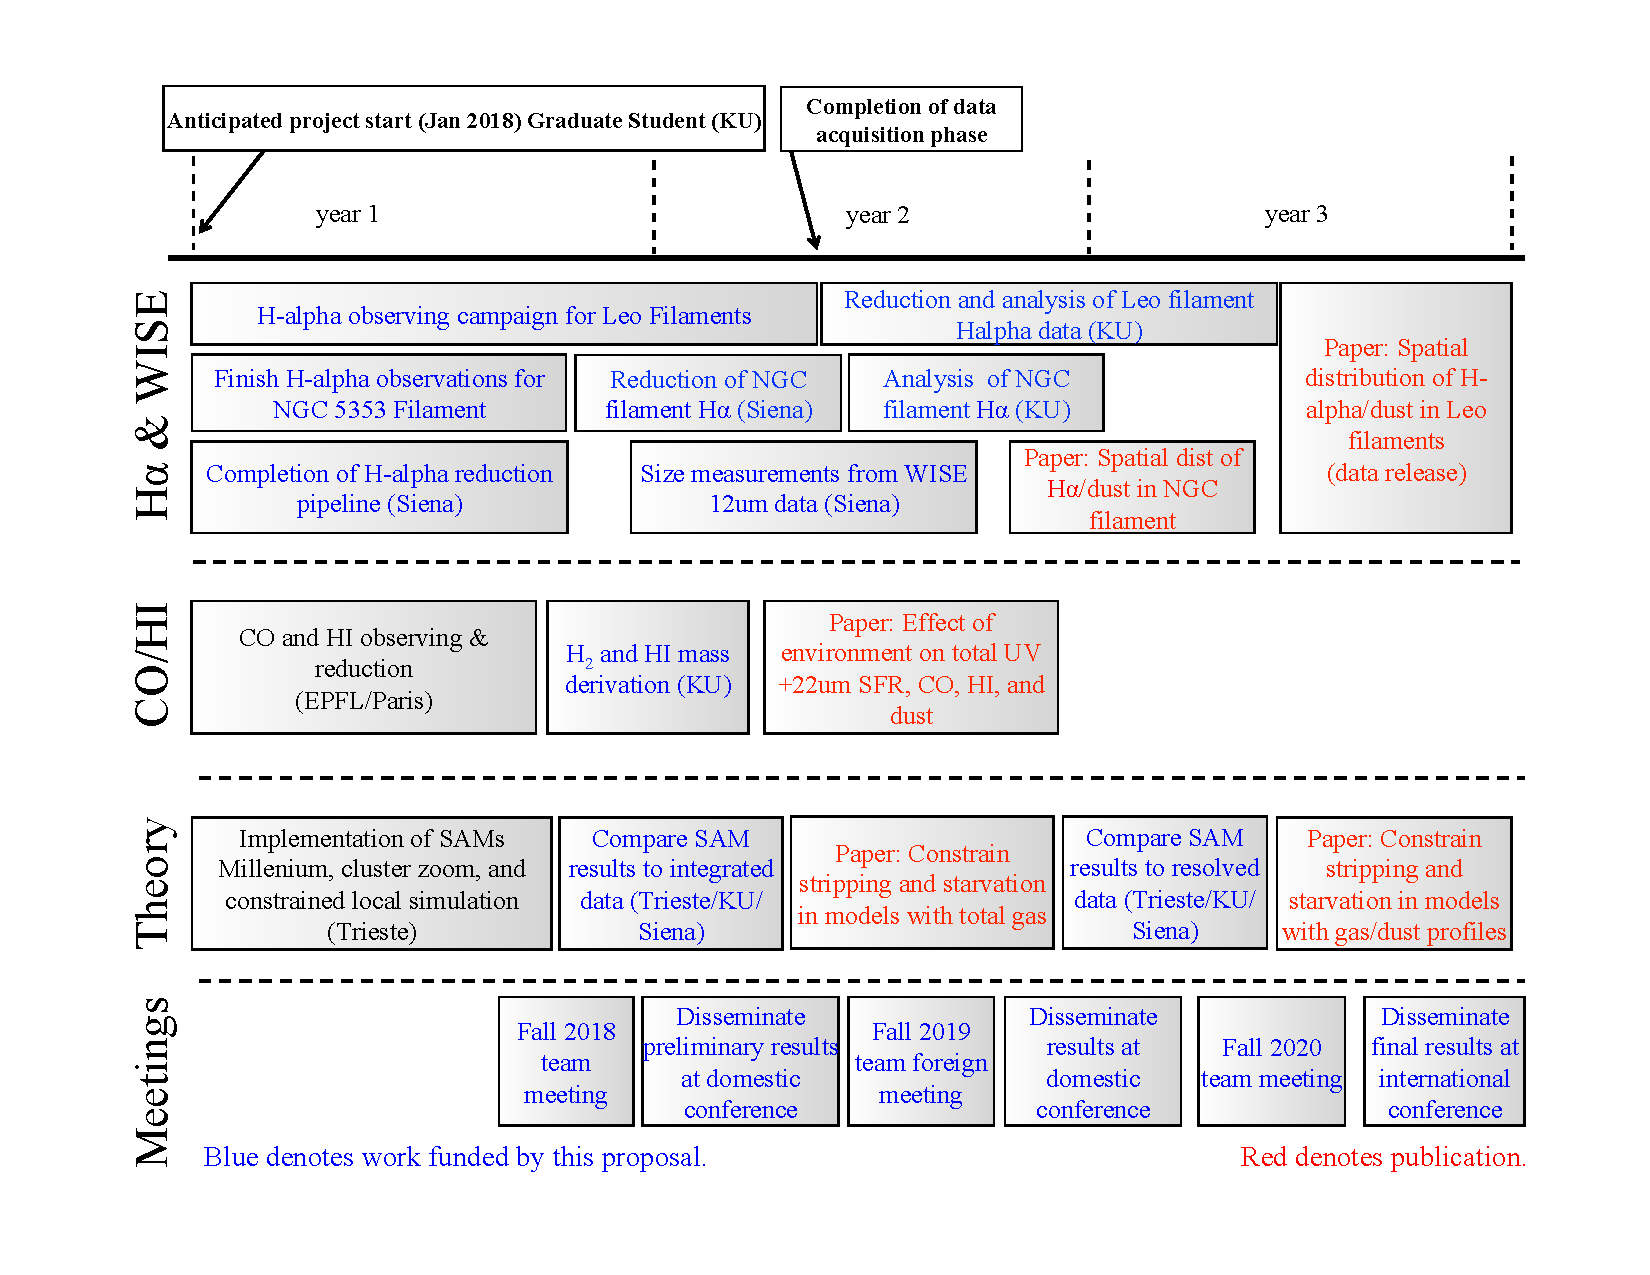
\includegraphics[width=1.1\textwidth]{work-plan2.pdf}
\vspace{-1.5cm}
\caption{Major Milestones and Timeline}
\label{fig:workplan}
\end{figure}

\vspace*{-.8cm}\subsection{Data Sharing and Further Dissemination of Results }
\vspace*{-.3cm}
%{\it To facilitate data sharing where appropriate, as part of their technical proposal, the Proposer shall provide a data-sharing plan and shall provide evidence (if any) of any past data- sharing practices.}

We will release all of our data with our final publication.  This will include 
reduced, calibrated, and astrometrically aligned
$H\alpha$ and dust maps, and with integrated CO and HI fluxes.
We will produce a catalog of CO, HI, dust, $H\alpha$
properties to be released with our final paper.
While this data set of derived information will not be exceptionally
large in volume, it will be of value to other observational
astronomers and theorists working on galaxy evolution. To facilitate
the widespread use of these data, we will publish the full catalog of
measured and derived quantities on the web and in the on-line version
of Astrophysical Journal Supplement. In addition, we will work with
the NASA/IPAC Infrared Science Archive (IRSA) to ensure that our data are
discoverable to a larger user base. Co-I Vandana Desai, resident at
IPAC, will act as our NED liason to ensure that this gets done in a
timely manner.

\vspace*{-.8cm}
\section{Results from Previous NSF Projects}
\vspace*{-.2cm}

Co-PI Finn has no prior NSF support to report.
\vspace*{-.8cm}
\label{Sec:prior_rudnick}
\subsection{Molecular Gas in Distant Galaxies (PI Rudnick)}
\vspace*{-.4cm}

Co-PI Rudnick has recently completed his NSF project 1211358
``Characterizing the Molecular Gas Contents of High Redshift
Galaxies'' (\$306,754; 8/1/12-7/31/16).  

\textbf{Intellectual Merit:} This study was based on a large body of
JVLA data (200 hrs) on a $z=1.62$ galaxy cluster that was collected
between 2012 and October of 2014. The goal of this study was to
characterize the molecular gas content of high-$z$ galaxies by
observing CO. As a result of the studies of this cluster and of the CO
gas content of distant galaxies, Rudnick has authored or co-authored
seven papers since 2012 with a total of 185 citations
\citep{papovich12,rudnick12,lotz13,geach13,wong14,geach14,tran15} as
well an ApJ paper that is in the resubmission process (Rudnick et
al.).  Since 2012, Rudnick has also given 28 oral presentations on
this NSF project.
%
Using the full JVLA data, Rudnick has securely detected CO(1--0) in
two massive and gas-rich galaxies in the $z=1.62$ cluster. These
galaxies have surprisingly low star formation efficiencies (SFE) for
their high mass and gas fraction \citep[e.g.][]{genzel10}. This may
indicate the presence of environmental effects on the physical
conditions of the molecular gas and on the accretion of gas from the
cosmic web in a massive halo. These results appear in a paper that is
being resubmitted to ApJ after a favorable referee report.  The
expected publication date is early 2017.  As a direct result of this
project Rudnick has also organized a large consortium of scientists
who are seeking to use ALMA to make a census of the CO gas in distant
cluster galaxies.  They will resubmit a significantly sized proposal in
April 2017.

\textbf{Broader Impact:} Rudnick has completed the third year
(2013-2016) of an outreach program in close collaboration with Andrew
Bricker, a Physics teacher at Lawrence High School (LHS). Rudnick
developed and executed a year-long program in which the students
receive an introductory calculus-based astronomy course and perform a
bona fide research project. The goal of the class is to teach high
school students research methods, computing skills, the
electromagnetic spectrum, the nature of science, and science
communication while also giving the teacher new tools to teach
research-based activities in the classroom.  The project involves
using \textit{Spitzer}/MIPS 24\micron\ data to measure L$_{\rm IR}$
and SFRs for the galaxies in the infall regions of intermediate
redshift clusters from the ESO Distant Cluster Survey (EDisCS). The
students meet every day in a special class period. The teaching
assistant funded by the grant performed most of the instructional
duties and Rudnick attended class once a week.  30 students have gone
through the program during these three years.  This total was
comprised of $\sim 50\%$ underrepresented student groups: four African
American, three Hispanic, one Native American, and 10 female students,
two of which were also women of color.  As described in \S\ref{BI} we
employ extensive assessment to understand our success at meeting
learning goals.  This program is continuing in 2016-2017 funded by
another NSF project (see \S\ref{Sec:gogreen_prior}).

\vspace*{-.7cm}
\subsection{Galaxy Evolution in Distant Clusters (PI Rudnick)}
\vspace*{-.4cm}
\label{Sec:gogreen_prior}

co-PI Rudnick is in the beginning of his second year for the NSF
project 1517815, ``Collaborative Research: The GOGREEN Survey - Caring
About the Environment'' (\$347,556; 8/1/15-7/31/18).

\textbf{Intellectual Merit:} This study funds the US analysis efforts
for the international Gemini Observations of Galaxies in Rich Early
Environments (GOGREEN) project.  This project is based on the largest
Gemini Long and Large Program (PI: Michael Balogh), which is comprised
of 443 hours of Gemini imaging and spectroscopic observations
conducted over a 4 year period starting in Fall 2014.  The two main
components of this project are very deep Gemini optical spectroscopy
of a stellar mass ($M>10^{10}M_\odot$) limited sample of galaxies in
21 groups and clusters at $1<z<1.5$ and a large multiwavelength
imaging program. 

The goals of the project are to: \textbf{1)} Find the dominant modes
of satellite quenching at $z<1.5$; \textbf{2)} Determine how galaxies
populate dark matter halos as a function of environment at $z<1.5$;
\textbf{3)} Measure the relative timing of morphological
transformation and star-formation quenching; \textbf{4)} Constrain the
dominant driver of size growth in the early-type population at
\boldmath$z<1.5$.  

co-PI Rudnick is in charge of the imaging efforts for the whole
collaboration, which involves gathering 11-band photometric data on a broad suite of
telescopes including Subaru, CFHT, Magellan, VLT, and $Spitzer$.  The
imaging of the southern clusters is 95\% complete and the northern
clusters only lack their NIR data.  We expect the imaging to be
completed by the Fall of 2017.

This ongoing project has not yet produced any publications.  The strategy of the project is to obtain deep spectra over many
semesters on the faintest targets, and thus many of the science
publications will appear at the end of the proposal period.  However,
an initial data paper based on the first 30\% of the spectroscopic
data is in preparation with a Dec. 2016 submission target.

\textbf{Broader Impact:} Rudnick has extended his LHS outreach program
into the 2016-2017 academic year and will continue it through the
2017-2018 AY.  Changes that we have made this year include a much more
agressive targeting of URM students, which we have accomplished by
going to more junior students and not having as high of a math
prerequisite for entry into the program.  As a result we have our
highest fraction of URM students yet, with one Native American, three
African American, two Hispanic students and three women ,one of which
is a women of color.  We are currently attempting to expand the
program by using seniors who have already completed the program as
peer instructors.  This will allow us to grow without additional
personnel costs.

\vspace*{-.7cm}
\section{Broader Impact}

\vspace*{-.4cm}
\subsection{Siena College}
\vspace*{-.4cm}

{\bf Modeling Physics for High School Programs:  }
The modeling
approach is an innovatve and effective way to teach physics that is 
fundamentally different from traditional techniques.  Students are led through
carefully constructed experiments and exercises to clearly develop the conceptual, 
visual, and mathematical models of how physics works.  
%Experienced physicists already have these mental models, 
%but beginning physics students do not.
These models are essential for understanding physics.
The modeling approach minimizes lectures, and instead 
students are actively engaged in collecting and analyzing real-time data
that illustrate the fundamental concepts of physics.   The students must
then construct models to interpret these
data.  

As a former high school teacher, co-PI Finn knows first-hand the importance of 
bringing the more effective and engaging techniques to the front line.
As part of a previous NSF grant (AST-0847430), we have offered 
modeling workshop for high school physics teachers for the past 9 summers.
We are fortunate
to have as an adjunct instructor an area high-school physics teacher who
is an expert in using the modeling approach to teach physics, and
he will continue to lead these 4-day workshops each summer.  
We offer continuing education credit to participants 
that can be used toward teacher recertification.
This grant will provide a stipend for Darren Broder to organize and lead
the workshops.  
To assess the impact of the modeling curriculum, participating teachers
will administer the force concept inventory and mechanics baseline test.

%Each spring, the School of Science will help sponsor a dinner for area math and
%science teachers.  The goal of this is two-fold.  First, we will have a Siena student
%present on a recent research project so that the teachers become better acquainted with
%the opportunities for Siena students.  Second, the teachers will have time for informal
%conversations to exchange teaching ideas and materials.

{\bf Undergraduate Research  :}
The importance of undergraduate research is widely recognized
in the science community.
{\em Recent studies have shown that undergraduate research may be the
pedagogy for the 21$^{st}$ century (e.g., Council on Undergraduate Research
Statement and references therein).}
Involvement in research projects
fosters highly motivated, self-confident students with enhanced
analytical and communication skills. 
co-PI Finn supervised 24 undergraduate students during the tenure of her
previous NSF grant (AST-0847430).

%The other member institutions are Colgate University,
%Cornell University,
%George Mason University,
%Georgia Southern University, 
%Humboldt State University, 
%Lafayette College, 
%St. Lawrence University, 
%Skidmore College, 
%Union College, 
%University of Puerto Rico, 
%University of Wisconsin, 
%Wesleyan University, 
%and West Texas A\&M University.
% As a team member, myself and participating Siena students
% have attended (Jan. 2008) and will continue to attend the Annual 
% Undergraduate ALFALFA Team Workshop at 
% Arecibo Observatory.  The workshop provides the framework for the program,
% communicating ALFALFA science, observing, and data analysis techniques to
% undergraduate researchers. During the workshop, lectures, observing sessions, and group work 
% are led by %National Astronomy and Ionosphere Center (NAIC)
% %staff, 
% team faculty and graduate students.  
% Siena members will also observe at Arecibo at other times during the year, giving students hands-on experience 
% in using a world-class national facility. 
% In addition, an NSF grant to support the undergraduate consortium has 
% provided money for Siena to purchase a dedicated computer for processing 
% ALFALFA data.  The same NSF grant will provide summer salary for one Siena 
% student every other year.
% However, more students are interested in participating, and therefore, we need more support.

%Previous Siena undergraduate students have worked on \ha \ imaging of
%nearby galaxy groups.  Together we have developed software to
%streamline the reduction process.  Students have presented their
%preliminary results at Siena's internal academic celebration, the fall
%meeting of the Astronomical Society of New York, and this January at
%the winter AAS meeting.  The proposed  work will benefit directly from
%the experience of my current undergraduate students and the software
%they have developed.

Siena College undergraduate students will be involved in all aspects
of this proposal.  We have budgeted money to bring students on
observing trips to Kitt Peak National Observatory, and they will help
gather imaging data at PCT through remote observing once the telescope
has been commissioned in the Spring of 2017.  This grant provides funds for four
undergraduates to complete 10 weeks of paid research for each year of
the grant.  Finn has experience supervising undergraduates on similar
projects, and hiring a mix of freshmen through juniors has worked
nicely as the older students can help train the freshmen.  
During the first year, two students will work with Finn to
finalize the data reduction pipeline for the KPNO data and to adapt
the pipeline for the TCP data.  The students will measure radial
profiles for the \ha\ imaging and develop ways to quantify the \ha\
morphologies.  The students will work in collaboration with the
graduate student at Kansas to compile the \ha\ data products.

The other two summer students will work on the analysis of the WISE
12\micron \ images.  This part of the project will require more
programming skills, and will likely be assigned to the more
experienced undergraduate students.  The students will work with Finn
and Vernizzi to analyze the images with GALFIT and visualize the
results of the multiple models that we will fit to each galaxy.

%Four Siena students began the first stages of their research projects this summer,
%and I expect all of these students to continue their involvement through the next academic year.
%Graduating students will be replaced by interested freshman or sophomores to maintain a total
%of 4 undergraduate researchers at any one time.  
%Specific goals for current and future student researchers are:
%\vspace*{-.2cm}
%\begin{itemize}
%\vspace*{-.25cm}\item learn how to use python for image reduction and
%analysis 
%\vspace*{-.25cm}\item learn how to effectively present their results to expert and
%non-expert audiences
%%\vspace*{-.25cm}\item learn how to reduce the radio data taken with the Arecibo Radio telescope
%%\vspace*{-.25cm}\item identify sources of Hydrogen emission and characterize the properties of the Hydrogen emission, such as the total mass of Hydrogen gas
%%\vspace*{-.25cm}\item cross-correlated the Hydrogen sources with existing surveys such as the Sloan Digital Sky Survey and the 2 Micron All Sky Survey
%\vspace*{-.25cm}\item identify correlations between \ha, infrared, and
%cold gas properties of galaxies and look for variations in these correlations as a function of galaxy environment.
%\end{itemize}
%\vspace*{-.2cm}


An important part of the research experience is presenting results
to the community. I will encourage all students 
to present their results at the fall meeting of the 
Astronomical Society of New York and Siena's Academic Celebration, which
is held each spring.  In addition, seniors will be encouraged to
present a poster at the 
annual winter meeting of the American Astronomical Society.  

To assess the impact of this project, I will track participation, papers, 
presentation, and post-graduate activity of all Siena students
who are involved in this project.  I will design and implement a survey to 
assess student plans/goals before, during, and after
participation in research.

\vspace*{-.8cm}
\subsection{University of Kansas}
\vspace*{-.4cm}
\label{BI}
\noindent \textbf{A High School Research Program:} Rudnick's broader
impact provides for the continuation of a successful research-based
outreach component at Lawrence High School (LHS; see
\S\ref{Sec:prior_rudnick}) that is funded by NSF proposals (1211358 and 1517815). This program is timely, as the Kansas
school system is an exemplar of the nationwide debate on the role of
science in the classroom. Crucial to increasing and clarifying the
role of science is educating students and training teachers.
%% What has become clear after the first year of this program is the
%% great value in bringing expert instructional support into the
%% classroom, as the partnering high school teacher lacks the research
%% experience at this point to adequately lead the program. The KU
%% employee (an ex-student) who is carrying out most of the in-class
%% instruction is proving crucial in this role. 
This program is currently funded through the end of the 2017-2018
academic year. The purpose of the current proposal is to: 1) continue
the funding of a KU student to work in the classroom, 2) develop the
project to the point of sustainability by training the high school
teacher in research-based teaching methods, 3) develop a peer
instruction model to expand the program to 20 students without
additional personnel costs, and 3) expand the program to 20
students. The school district fully supports this program (see letters
from McEwen and Bricker.)

Students in this program have carried out a multitude of research tasks, including cross-matching of multi-wavelength catalogs, understanding the relation between catalog and image-level data, measuring SFRs from 24\micron\ fluxes, computing cluster-averaged properties such as integrated SFRs, comparing results from different groups, assessing the validity of their results, and presenting the results in written and oral form.

\noindent \textbf{Implementation:} LHS has a 60\% higher percentage of
African Americans and a 340\% higher percentage of Native Americans,
when compared to other Kansas High Schools. Rudnick will continue his
successful recruitment of female students and those from
underrepresented minorities. The current proposal will extend the
ongoing project to measure SFRs of galaxies in the local filaments.
%% Coupled with student measurements
%% being made of EDisCS clusters at $0.4<z<0.8$, this will allow the
%% students to constrain the evolution in the SFRs of cluster galaxies
%% from $0.4<z<1.5$.
The requested funding will be used to continue employment for the current outreach coordinator Brian Schafer, who is an ex-KU Astronomy, Physics, and Chemistry undergrad with extensive teaching training and now four years of experience with our outreach program.  This employee will be the main contact person in the
classroom and will lead the day-to-day instruction and supervision of
the learning teams during the execution of the project. co-PI Rudnick's role is to coordinate the program, decide on the exact
curriculum modifications based on our assessment process (see below), attend the
class once every week, and ensure that the program becomes sustainable
in future years. Through Rudnick's \textit{continuous} support and
heavy involvement in the program, the high school teacher is able to devote more of his time to training students to aid in peer instruction, which will allow us to expand in future years without additional personnel costs.

%% The KU graduate program has a solid record of students with an
%% education background or with an interest in education and outreach.
%% Rudnick currently has an ex-student employee who is excelling in his
%% role, but if needs be there will no problem recruiting a new student
%% with the necessary skills and motivation.

\noindent
\textbf{Assessment:} %% The program has been constructed according to the
%% theory of backwards design, in which the broad goals are defined
%% first, then specific goals, followed by the means of assessment, and
%% finally the details of implementation. The goals and implementation
%% are outlined in the previous paragraphs. 
The assessment consists of an end of project presentation and paper
for each student. Their presentations are made to KU faculty during a
mini-conference at KU. All students are given the pre- and post-course
Light and Spectra Concept Inventory \citep{bardar06}.  We also make
students give multiple oral presentations throughout the semester and
have a rubric to evaluate their improvement over the course of the
project.
%% One ongoing task of the employee will be to research and develop
%% new assessment tools and to modify the program accordingly to the
%% results. As an example, in the Fall of 2014, Rudnick has decided
%% to focus more
%on student presentations in the astronomy instruction part of the
%course, to give the students practice in actively seeking out and
%presenting their own astronomy knowledge.
This project satisfies important elements of several of the Kansas
state science standards, i.e.~``Science as Inquiry'' via the process
of research and of communicating their results, benchmark 2 and 3 of
the Physics standards via learning about the electromagnetic spectrum
and how it relates to astronomical phenomena, benchmark 4 of the earth
and space sciences standards relating to general astronomy, and
benchmark 2 of the ``history and nature of science'' via the
understanding gained of the scientific process.




\clearpage
\bibliography{rfinn,nsfCAREERref14,clusters,references_2,HSTreferences}
%\bibliography{/Users/rfinn/bin/bibtex/rfinn}
%\bibliographystyle{nsf}
\bibliographystyle{nsf}
%\bibliography

% NOTES:

% look at star formation in dwarfs

% halpha luminosity function

% post-bac student to reduce Halpha

% write reduction pipeline

% summer salary

% filter for Mt Laguna - 

% travel funding for conferences
% group meetings 


% models from Gabriella

% letters of support from Gabriella, Pascale, Francoise


% Halpha + CO - grant 
% size of SF region in different 

% THEORY:
% - spatial distribution of Virgo-like cluster
% - illustrus hydrodynamical simulations
% - compare with CLUES - simulations of local volume


% select sample - determine the amount of observing time required.



% filaments - 

% literature with existing CO observations

% Young+1995
% Brain, Combes + 93
% Sage 93
% Casoli+98
% HERACLES, IRAM CO(2-1)
% ATLAS 3D - Young+2011
% BIMA-song

% filament 3 - 


% Cosmic flows:
% Tully; Courtois

% CLUES - simulations; gas stripping, size of SF region, gas mass (below
% 1E4 K)

% post-processing - compute amount of mass that has been stripped;

% fund:
% observing;
% filter;


\end{document}
